\documentclass[4apaper,12pt]{book}
\usepackage{amsmath}
\usepackage{index}
\usepackage{gensymb}
\usepackage[toc,page]{appendix}
\usepackage{hyperref}
\usepackage[semicolon,round,sort&compress,sectionbib]{natbib}
\usepackage{graphicx,accents}
\usepackage{chapterbib}
\usepackage{tikz}
\usepackage{pgfplots}
\usepackage{subcaption}
%\usepackage[demo]{graphicx}
\pgfplotsset{width=10cm,compat=1.9}
\usepgfplotslibrary{external}

% Define \figref as abbreviation of "Figure~\ref{...}"
\newcommand\figref{Figure~\ref}
%\usetikzlibrary{positioning}
\usetikzlibrary{positioning, fit, arrows.meta, shapes, chains}

% used to avoid putting the same thing several times...
% Command \empt{var1}{var2}
\newcommand{\empt}[2]{$#1^{\langle #2 \rangle}$}

\makeindex



% for mathematical symbols
%\usepackage{amsfonts}
\usepackage{amssymb}


\begin{document}

\title{AI and Machine Learning mathematics  with algorithmic implementation}
\author{mohab metwally}
\date{2020}

\maketitle
\tableofcontents

\chapter*{Introduction}
\addcontentsline{toc}{chapter}{Introduction}

\section{notation}
\begin{description}
  \item through the book i sometimes use subscript without braces, or superscript with braces, or even curly braces to indicate vector element access, or row access in the case of a matrix.
\item $(x, y) \in R^{n_x}, y \in {0,1}$ are the training data-set, where x is input,  and y is corresponding output.
\item therefore $M=\{(x^1, y^1), (x^2, y^2), ..., (x^{m}, y^{m})\}$  is the training set, and $M_{test}$ is test example.
\item X is the input of training set and $\in R^{n_x \times m}$, $X=\begin{vmatrix}X^1&X^2&...&X^{m}\end{vmatrix}$, $X^{(i)}$ is the ith column of length n, and can be written as x, or $x^{(i)}$.
\end{description}

\chapter{Logistic Regression as a neural network}

\section{definitions}

\begin{description}
\item we need an estimate function $\hat{y}$ for the input x, and weight prameters w$\in R^{n_x}, b\in R$.
\item logstic function is $\hat{y}=p(y=1|x)$, and can be defined as follows: $\hat{y}=\sigma(w^Tx+b)$, where the sigma function is defined by $\sigma(z)=\frac{1}{1+e^{-z}}$, and notice when z $\to \infty, \sigma = 1, z \to -\infty, \sigma =0$.
\item
\end{description}

\section{cost function}

\begin{description}
\item starting with a estimation linear forward model $\hat{y}$, we calculate the difference between our estimate, and the real value $y$, and through optimization we try to minimize the difference, or loss/cost through gradient descent, then we update our model's parameters.
  \item loss function is minimizing the difference between estimation ${\hat{y}, y}$, and can be defined as least squre $L(\hat{y}, y)=\frac{1}{2}(\hat{y} - y)$, but least squares leads to non-convex loss function(with multiple local minimums).
\item there are different loss functions, but the most efficient is that which maximize the difference. we can define $P(y|x^{(i)}, \theta) = h(x^{(i)},\theta)^{y^{(i)}}(1-h(x^{(i)},\theta)^{1-y^{(i)}}$, to increase the sensitivity to the training set we take the likelihood function, as the loss, $L(\theta)=\prod_{i=1}^mP(y|x^{(i)}, \theta)$ see $\mathbf{(AppendixA)}$.
\item one final step in our model is that as m get larger L tend to go to zero, to solve this we define the average sum of log-likelihood, or loss function to be our Cost function.
\item we multiply by -1 since the sum of the log-likelihood function is negative.
\item the Cost function  $J(\theta)=\frac{1}{m}\sum_{i=1}^{m}log(h(x^{(i)},\theta)^{y^{(i)}}(1-h(x^{(i)},\theta)^{1-y^{(i)}})$

\item loss function is defined as $L(\hat{y}, y)=-[ylog(\hat{y}) - (1-y)log(1-\hat{y})]$, L$\in[0-1]$.

\item cost function is defined as the average of loss function $J(w,b)=\frac{1}{m}\sum_{i=1}^{m}L(\hat{y^{(i)}}, y)$
\end{description}

\section{Gradient Descent}

\begin{description}

\item gradient descent is a way to tune the weighting parameters, the objective is the lean toward the fittest weights with respect to the least cost.
\item iterate through cost function $\mathbf{J}$ tuning with respect to weight parameters  $\mathbf{w}$, $\mathbf{b}$.
\item iterate through: $w:=w-\alpha\frac{\partial{J}}{\partial{w}}$,  $b:=b-\alpha\frac{\partial{J}}{\partial{b}}$, for tuning w, b for the least $\mathbf{J}$ possible, such that $\alpha$ is the learning rate of GD.
\item for simplicity $\partial{J}/\partial{w}$ replaced for $\partial{w}$, and similarly $\partial{J}/\partial{b}$ is replaced for $\partial{b}$.
\item forward propagation, $$\partial w = \frac{\partial{J}}{\partial{L}}\frac{\partial{L}}{\partial{\hat{y}}}\frac{\partial{\hat{y}}}{\partial{z}}\frac{\partial{z}}{\partial{w}}$$, similarly $$\partial b = \frac{\partial{J}}{\partial{L}}\frac{\partial{L}}{\partial{\hat{y}}}\frac{\partial{\hat{y}}}{\partial{z}}\frac{\partial{z}}{\partial{b}}$$.
\item $$\partial{L}/\partial{\hat{y}}=\frac{-y}{\hat{y}} + \frac{(1-y)}{1-\hat{y}}$$, $$\partial{\hat{y}}/\partial{z}=\frac{-e^{-z}}{1+e^{-z}} = \hat{y}(1-\hat{y}).$$
\item $\partial{L}/\partial{z}=\hat{y}-y$.
\item then we can deduce that the final iteration gradient descent step after calculating sigma, loss, and cost functions can be  $$w:=w-\frac{\alpha}{m}\sum_{i=1}^m\frac{\partial{L}}{\partial{b}}=\frac{\alpha}{m}X^T(\hat{y}-y)$$, and $$b:=b-\frac{\alpha}{m}\sum_{i=1}^{m}(\hat{y}-y)$$.
\end{description}

\section {Model training}
\begin {description}
\item to train a logistic regression model given data set of \textbf{{X,y}} we divide it into 20\% for testing, and 80\% for training, such that the training set is used to train our model parameters, and testing set is a separate set to test our model's predictions.

\item we call $X=\{X_{training},X_{testing}\}, y=\{y_{training},y_{testing}\}$ the data set, and
  $\{X_{training}, y_{training}\}$ the training set,and
  $\{X_{testing}, y_{testing}\}$ the testing set.
\item using $X_{training}, y_{training}$ (for the rest of the chapter, and the book i will refer to them by $X,y$ for simplicity) we start \textbf{Forward propagation} to estimate $\hat{y}$ calculate the difference between $y$, $\hat{y}$ through \textbf{Cost function} $J(y,\hat{y})$.
\item going backward to W, b we implement \textbf{Backward propagation} through $\frac{\partial{J}}{\partial{\omega}}$, and $\frac{\partial{J}}{\partial{b}}$.
\item finally we \textbf{update weight parameters} after sufficient iterations until we minimize our cost function completely.
\end {description}

\section{Forward Propagation}
\begin{description}
\item we begin by initializing our weight, and bias parameters
  $\omega$, b randomly.
  \subsection{Activation Functions}
  \item what is activation function?
\item sigmoid:
\item relu:
\item tanh:

\item Starting with input training set \textbf{X} in our model. we estimate
  $$z=\omega^TX + b$$. then $$\hat{y}=\sigma(z)$$.

\item calculate cost function $$J(y,\hat{y})$$.
\end{description}

\section{Backward Propagation}
\begin{description}
\item after evaluating the cost function $J(y,\hat{y})$ we calculate it's derivative with respect to  $\{\omega,b\}$.

\item $$\partial{\omega}= \frac{\partial{L}}{\partial{\omega}}=
  \frac{\partial{L}}{\partial{\hat{y}}}
  \frac{\partial{\hat{y}}}{\partial{z}}
  \frac{\partial{z}}{\partial{\omega}}$$
\item $$
  \frac{\partial{L}}{\partial{\hat{y}}} = -
  (\frac{y}{\hat{y}} - \frac{(1-y)}{(1-\hat{y}}) =
  \frac{\hat{y}-y}{\hat{y}(1-\hat{y})}
  $$

\item $$e^{-z}=\frac{1}{\hat{y}} - 1=\frac{1-\hat{y}}{\hat{y}}$$
\item $$
  \frac{\partial{\hat{y}}}{\partial{z}} =
  \frac{e^{-z}}{1+e^{-z}} = (\hat{y})^2e^{-z}
  $$
\item $$ \partial{\omega} = X^T(\hat{y} - y) $$
\item $$ \partial{b} = \hat{y} - y $$
\end{description}

\section{Update parameters}
\begin{description}
  \item we implement the following algorithm with a fixed number of iteration that is customized per application, and tuned by the Engineer, such that each application would require different tuning parameters from which is the iteration number.
\item we iterate the following: update the parameters $\omega$, b, in the back propagation step using $\partial{\omega}$, $\partial{b}$.
\item $$\omega = \omega - \frac{\alpha}{m}X^T(y-\hat{y})$$
\item $$b = b - \frac{\alpha}{m}(y-\hat{y})$$

  \end{description}

\section{Summary}
\begin{description}
  \item
\end{description}

\section{Logistic Regression in Python}
\begin{description}
  \item
\end{description}

\section{References}
\begin{description}
  \item
\end{description}

\chapter{Neural Networks}
\section {Lingua franca}

\begin{itemize}
\item RELU Activation Function: It turns out that using the Tanh function in hidden layers is far more better. (Because of the zero mean of the function). Tanh activation function range is [-1,1] (Shifted version of sigmoid function). Sigmoid or Tanh function disadvantage is that if the input is too small or too high, the slope will be near zero which will cause us the gradient decent problem. RELU stands for rectified linear unit, it's a rectifier Activation function and can be defined as $f(x)=x^+=max(0,x)$ or $\begin{cases} 0 & x\leq 0 \\ x & x > 0 \end{cases}$ relu shows to be better replacement to sigmoid function $\sigma$ for the reason that it help in vanquishing gradient problem.
\item Neuron: is a linear regression algorithm denoted by z, or a, $z= W^TX + b$, such that W is the the weight vector of the network.
\item Shallow Layers: also known as Hidden Layers, is a set of neurons, for example of the network of composed of input $X$, and output $Y$, with at least a single layer $L1$, and at most 2 layers, then the forward propagation will be as follows: we calculate the logistic function for the first layer $(1)$,  $z^{1}_i=w^TX_i+b_i$, $\hat{Y}^{(1)}=\sigma{(z^{1}_i)}$ , then we proceed to calculate the final logistic evaluation for the output layer with $\hat{Y}^{(1)}$ as an input instead of $X$, and so on we proceed replacing $\hat{Y}^{(i)}$ instead of X as new input.
\item Layer: layer $L_{(i)}$ is $\hat{Y}^{(i)}=[\hat{y}^{(i)}_1, \hat{y}^{(i)}_2, ..., \hat{y}^{(i)}_n]$ such that n is the length of the layer $L_{(i)}$. each $\hat{y}^{(i)}_{j}$ is weighted with unique weight vector with previous layer $L_{(i-1)}$.

\item Neural Network(NN): is a set of interconnected layers, $<X, L_1, L_2, ..., L_m, Y>$

\item Deepness: shallow layer as defined to consist of 1-2 hidden layers, but on the other hand Deep Network is consisting of more than 2 inner, or hidden layers.

\end{itemize}

\begin{description}
\item we discussed in previous chapter that $\frac{\partial{\hat{y}}}{\partial{z}}$, is actually for the logistic activation function $\sigma$ only, we need to calculate the same derivation for tanh, and RELU.
\item for $tanh(z)=\frac{e^{z}-e^{-z}}{e^{z}+e^{-z}}$ is $\frac{\partial{\hat{y}}}{\partial{z}}=1-tanh(z)^2$
\item for relu activation function $\frac{\partial{\hat{y}}}{\partial{z}}=\begin{cases}0 & z<0\\1 & z\ge0\end{cases}$
\item in NN there are plenty of parameters to worry about, for example the weights need to be initialized randomly, with small values, and $b$ can be initialized as zero.
\end {description}

\section{Model training}
\begin{description}
\item Training a deep neural network is analogous to training a logistic regression network, as discussed in previous chapter, a logistic regression model can be considered a neural network with zero \textbf{hidden layers}.
\item We follow the same algorithm, parameter initialization, but in this case we initialize the parameters for each layer, assume a network composed of 2 hidden layers $X \rightarrow L1 \rightarrow L2 \rightarrow Y$, layer $(L^{(i)}, L^{(i-1)})$ are interconnected with weight,bias parameters $\omega^{(1)},b^{(1)}$, such that $\omega^{(i)}$ is a matrix of shape $(length(L^{(i)}), length(L^{(i-1)})$, and $b$ is a vector of shape $(length(L^{(i)}, 1))$, so each node in the layer $L^{(i)}$ is connected with each node in previous layer $L^{(i-1)}$.
\item W, b are ought to be randomly initialized, in the logistic regression discussed in previous chapter, W, b should be initialized with zero values, but in the case of the neural network zero initialization leads to $\hat{y}=0$, and all the nodes share the same weight which violates the purpose of the nodes in the first place which is to capture features from the data set as much as possible, so random initialization is necessary, and not to overshoot, initialization better in range $]0-1[$ weighted by small value around 0.01(this will be discussed in details in NN hyperparameters chapter) to reduce the sensitivity, in order for the gradient descent to not take for ever.
  \item forward and back propagation are executed in a similar way to logistic regression with minor differences.
  \item calculation of forward propagation using inputs from the previous layer instead of input data set, activation function can be \textbf{sigmoid}, \textbf{relu}, or \textbf{tanh}, it has been tested that \textbf{relu} activation function in the first layers shows better results, and \textbf{sigmoid} activation in the last layer to fit perfectly with the output classification y-vector in the range $[0-1]$

\end{description}

\section{Parameter initialization}
\begin{description}
\item Iterating through each layer, such that $L^i$ layer of length $l_i$ nodes, and previous layer $L^{i-1}$ of $l_{i-1}$ nodes, the weight parameter at layer L is inter-connected with all nodes in the previous layer, meaning that nodes at layer $L^i$ ought to have weight matrix of shape $(l_i, l_{i-1})$, and bias of shape $(l_i,1)$.
\item Unlike the logistic regression, in Neural network initialization step is crucial step, in logistic regression there is only a single activation node extracting a single feature such as price of a house for example, but we intend to employ neural networks to capture as many features as possible inside each node, and therefor initialization ought to be with random values, otherwise we end up with similar copies of each node forward, and backward propagation.
\item and since we choose random $W^i$ we can choose $b^i$ to be zero.
  \subsection{Xavier initialization}
  \begin{description}
  \item randomizing weight parameters from a Gaussian, or normal distribution help to keep the initial values contained, or in other words, solves the vanishing, exploding gradient problem , instead to be demeaned around zero, this is proven to reduce variance (we will discuss this in details later on)
    \end{description}
\end{description}

\section{Forward Propagation}
\begin{description}
\item similar to logistic regression forward propagation, done for each layer, with little difference that instead of using sigmoid function $\sigma$ we replace it with \textbf{relu} function, which is shows better results, and activate the last layer with sigmoid function to distribute the output toward the extremes.
\item the forward propagation step is done on the input $A^{i-1}$ from previous layer, with current layer $L^i$ parameters $\omega^i$, $b^i$.
  \item we iterate through layers $L^i$ such that $i \in [0,L]$
\item  $$z^i=(\omega^i)^TA^{(i-1)}+b^i$$.
\item $$
  A^i=\begin{cases}
  \text{relu{($z^i$)} $\leftarrow$ if i $<$ L} \\
  \text{$\sigma(z^i)$ $\leftarrow$ if i = L}
  \end{cases}
  $$

\end{description}

\section{Backward Propagation}
\begin{description}
\item $$
  \frac{\partial{L^i}}{\partial{\omega^i}}=
    \frac{\partial{L^i}}{\partial{A^{(i-1)}}}
      \frac{\partial{A^{(i-1)}}}{\partial{z^i}}
        \frac{\partial{z^i}}{\omega^i}
        $$
      \item $$\partial{A^{(i-1)}}=\partial{z^i}
        (\frac{\partial{A^{(i-1)}}}{\partial{z^i}})^{-1}=
        \partial{z^i}\frac{\partial{z^i}}{\partial{A^{(i-1)}}}
        $$

      \item since the last activation function is sigmoid, then $$\partial{z^L}=y^L-\hat{y^L}$$
        \item the back propagation algorithm start with the following initialization step:.
        \item $$ \partial{A^{(L)}} = \frac{(\hat{y}-y)}{\hat{y}(1-\hat{y})} $$
        \item $$\partial{A^{(L-1)}} = (\omega^{(L)})^T(y^{(L)}-\hat{y^{(L)}})$$
        \item $$ \frac{\partial{z^i}}{\partial{A^{(i-1)}}} = \omega^T $$
        \item $$\partial{A^{(i-1)}}=\omega^T\partial{z^i}$$

\end{description}

\section{Summary}
\begin{description}
\item
\end{description}

\section{Deep neural networks in Python}
\begin{description}
\item
\end{description}

\chapter {Neural Networks hyperparameters}
\begin{description}
\item machine learning have a wide applications in ranging from Computer Vision, Natural Language Processing, Speech recognition, and structured data, in data-science, and the the parameterization varies greatly from one domain to another, it's domain specific.
  \subsection{training}
\item  given a data set, wide range of models, the data  data is divided into three categories, the \textbf{training}, \textbf{development}, and the \textbf{testing}.
\item we train different models to evaluate the most fit model on the development(also called evaluation set), after choosing our model we test on the testing set.
\item the partitioning ratio of the data-set varies with the size of the data set, for example in a small data set of size 1000, it's convenient to divide the data into 70\%, 30\% for training, and test respectively, or 60\%, 20\%, 20\% for training, evaluating, and testing respectively, but in the era of big data, of millions of entries, data set is conveniently divided into (98\%, 1\%, 1\%), (99.5\%, 0.4\%, 0.1\%) for training, evaluation, testing sets respectively, the ratio varies from one domain to another.
\item for faster, and accurate training/testing the data-set ought to be for the same source of the same general range of features, on the other hand in the mismatched data-set, in the case of training set from specific source, and development/test set from different set, the development/testing process can be inefficient, so the division of the partitioned sets need to be taken randomly from the same source.
  \subsection{bias-variance trade-off}
\item In an n-dimensional training model, the bias-variance dimension indicates how far our model captures the data, and can be classified into under-fitting high-bias model where it hardly fit the data, on the other extreme, high-variance, over-fitting model, and in between just-right model.
\item high-variance: in a classification problem where the training set error is 1\%, while the dev set error is 11\%, this gape indicate that the model is well trained in a very narrow data-set with limited range of features quite different from that of the development set, in this case the model is over-fitting, or hardly scaling to other data-sets, and therefore fails in application.
\item high-bias: similarly in the same experiment if the training set error is around 15\% where the dev-set error is ~ 16\%, indicating that the model generalize much better than the previous case of high-variance over-fitting model, but with high error would indicate that the model is highly-biased, and well generalized.
\item high-bias, high-variance: the worst model is that which do not generalize well, and doesn't fit our data, with high training error say 15\%, and 30\% development error.
\item low-bias, low-variance: the perfect model is that of low bias, low-variance, that which fits the training set, and generalizes well.
  \subsection{recipes for high-bias, high-variance}
\item high-bias solution: getting a high bias means that our model doesn't capture sufficient features, and this can be due to  our network is short, or narrow, or the gradient descend need to be run for longer time, or through using optimization, or change the neural network architecture.
\item high-variance solution: high variance indicate the lack of generalization, and is reduced through training on wider data-set, regularization, and changing the NN-architecture.

  \subsection {Regularization (weight decay)}
\item in the case of high-variance, we need our model be more generalized over the data-set, one way to do so is through regularization, or changing the sensitivity of the weight parameters, this sensitivity is measured in the back-propagation step through $\partial{J}/\partial{w}$, we can vary the sensitivity by regularization parameter $\lambda$ added to the cost function  as follows:
  $$ J(w^1,w^2...,w^L,b^L,b^L...,b^L) = \frac{\alpha}{m}\sum_{i=1}^{m}{L(w^1,w^2...,w^L,b^1,b^2...,b^L)} + \frac{\lambda}{2m} \sum_{l=1}^{L} {\left\Vert w^{i} \right\Vert^2}  + \frac{\lambda}{2m}b^L $$

\item but usually the last term is quite ineffective in regularization, and ignored, so it's cuts down to the following:

\item $$ J(w^1,w^2...,w^L,b^L,b^L...,b^L) = \frac{\alpha}{m}\sum_{i=1}^{m}{L(w^1,w^2...,w^L,b^1,b^2...,b^L)}  + \frac{\lambda}{2m}  \sum_{l=1}^{L} {\left\Vert w^{i} \right\Vert^2} $$

\item where the last norm is frobenius norm:
  $$ \sum_{i=1}^{n^{(l)}} \sum_{j=1}^{n^{(l-1)}} (w_{i,j}^{(l)})^2 $$

\item backward propagation step:

\item  $$ \frac{\partial{J}}{w^{i}} = \frac{1}{m}\sum_{i=1}^{m}{\frac{\partial{L}}{\partial{w^L}}}  + \frac{\lambda}{m}  \sum_{l=1}^{L} {\left\Vert w^{i} \right\Vert} $$

\item looking at our mechanism now, $\lambda$ is a device for tuning the weight parameter, or rather as a valve to control it, the larger the $\lambda$ is the lower the w as we minimize our cost function.

  \subsection {Inverted Dropout Regularization}
\item instead of reducing the weight parameters, we can drop it out completely by assigning those values to zero.
\item implementation algorithm: by matching a threshold probability = $P_{keep}$ against activation matrix $A^{(i)}$, and to keep balanced activation values, it's re-evaluated as $A^{(i)}/(1-P_{keep})$ and this last step distinguish the inverted dropout, from normal dropout, and the inverted is more efficient.

  \subsection{Input Normalization}
\item since there are no constraint on the input features, each feature can be of different range, and the cost function can end up elongated at one dimension, and narrow on the other, being steep on one edge of the function, and smooth on the other, it can be visualized by taking a contour of the \textbf{J} function, it will look like very long ellipse.
\item with un-normalized input the gradient descend tends to take long time, and longer way down to the local minima, but if the input is normalized (demeaned, and divided by the standard deviation of the input) we end up with circular counter, and smooth, and faster gradient descent.

\subsection{Vanishing/Exploding gradients}
\item let's look deeper inside a deeper network, through L layers, such that L is large, $\hat{y}=(W^LW^{(L-1)}W^{(L-2)}...W^1)X$ if we assume $b=0$ for simplicity, and that $W^L$ is the transpose of $w^L$, in case entries of similar weight matrices in values, if the values of each $W^i$ matrix below the 1, then the overall $(W^LW^{(L-1)}W^{(L-2)}...W^1)$ term will be very small, and gradient descent will take forever, on the other hand, if those entries greater than 1, then the overall term will be huge, and the gradient descend will overshot(exploding).

\item a well chosen initialization parameters can Speed up the convergence of gradient descent, and Increase the odds of gradient descent converging to a lower training (and generalization) error.

    %TODO name the formula, and elaborate.
\item to solve vanishing/exploding gradients problem we take two steps in weight parameters initialization, first the values are choosing at random through normal distribution, secondly, setting up the variance of $w^i$ to $\frac{1}{k}$  such that k is the number of the neurons in layer $i-1$. and it's by multiplying of $w^i$ by $\sqrt{\frac{1}{k}}$, this ratio shows to fit better with relu activation if replaced with $\sqrt{\frac{2}{k}}$

\item back to inverted dropout algorithm, due to the vanishing/exploding gradients problem we fix a threshold $P_{keep}$ and compare each entry in $W_i$ (taken from uniform distribution [0-1], unlike previously we choose W at random from normal/Gaussian distribution), so.
\item back propagation step we run the same masking algorithm over $\partial{A^{l}}$ and divide it by the same factor.
\item if $A^{l}=\frac{mask(A^{l})}{P_{keep}}=\frac{A^{l}.*A_{mask}}{P_{keep}}$, then $\partial{A^{l}}=\frac{\partial{A^{l}}.*A_{mask}}{P_{keep}}$ note that $.*$ means element-wise multiplication.
  \subsection {gradient checking}
  \item we verify the GD isn't converging.
\item it's a method to verify that the gradient descent is within diminishing $\epsilon$ of error difference with the manual derivative of the derived function $f(\theta)$, and $\theta$ is a vector of unwrapped weight, and bias parameters.

\item if following the Euclidean distance $L_2$ norm difference $ < (\epsilon =10e-7)$ then the result is negative. $$
  \frac{
    \left\Vert\frac{\partial{J(\theta^i)}}{\partial{\theta^i}} - \frac{\nabla {J(\theta^i)}}{\nabla{\theta^i}}\right\Vert
  }
       {
         \left\Vert\frac{\partial{J(\theta^i)}}{\partial{\theta^i}}\right\Vert +
         \left\Vert\frac{\nabla{J(\theta^i)}}{\nabla{\theta^i}}\right\Vert }  < \epsilon $$
\end{description}

\section {Optimization}

\begin {description}
\item machine learning is highly iterative process, to choose low-bias, low-variance model from the set of trained/tested models, the iteration process for each model through the same m data-set entries, of L layers, and this process is time consuming, optimized algorithms are essential.
  \subsection{stochastic, mini-batch, and batch gradient descent}
\item let's consider the input data-set $X$ of image-classification model Neural Network, using big-data of 5 million images, each with resolution of $800*400$, and three color channels, then our input Matrix X would be of size $5M*800*400*3$ bytes need to be loaded in the training machine memory, that is around 4.37 Tera bytes!
\item to be able to train our model we divide our Input set into mini-batches, if we choose the batch size to be 1 meaning we run the gradient descent on a single input entry, without taking benefit of vectorization, and machine GPU, then it's called \textbf{stochastic gradient descent} it's a \textbf{mini-batch} of size 1, even using input from the same distribution the cost function hardly reduces to the local minima, and tend to take random-walks for each input, it's hard to predict it's behavior, but for the overall training-set it converges to the neighbourhood area of the local minima. but on the bright side it can run on a moderate computer, but takes longer time compared to \text{batch gradient descent} that make full use of vectorization, and GPU power.
\item if we take the benefits of both worlds and choose \text{mini-batch} size fit enough to run in our training machine GPU/CPU memory, we can run our model in the  optimal time possible. so instead of running (X,Y) of size $m$ inside our model, we divide our training data-set (X,Y) into $(X^{\{t\}}, Y^{\{t\}}) | t=\frac{m}{number-of-batches}$ mini-batches.

\end{description}

\section{Gradient descent with momentum}
\begin{description}
\item  In the case of min-batch gradient descent, or in slow gradient descent the descent tends to overshoot, and deviate from the shortest path, to solve overshooting we employ weighted averages of the gradients (see appendix (D) on exponentially weighted averages) as follows: $$ Vdw^i = \beta_1 Vdw^{i-1} + (1-\beta_1) dw^i $$
\item then we use $Vdw^i$ in update parameters step, $w^i = w^i - \alpha Vdw^i$.
  \end{description}

\section{RMSprob}
\begin{description}
\item In a highly oscillating converging gradient descent around the axis of convergence, we can employ 'root mean squared prob' algorithm also using weighted averages, and here is the formula $$ Sdw^i = \beta_2 Sdw^{i-1} + (1-\beta_2) (dw^i)^2 $$, the only difference here is that the last term's parameter is squared, and it's useful in the case of oscillating gradient along side an axis perpendicular to the converging axis, the squared weight will boost relative large value, or shrink down relatively small value, then in the update step we divide by the square root of the calculated maximized/shrinked weight value, if it was initialize relatively small we can compensate by increasing the learning rate $\alpha$ to leap larger steps, if the initial $dw$ value was relatively large then we shrink it for more stable gradient descent.
\item the last step is: $$ w^i = w^i - \alpha \frac{dw^i}{\sqrt{Sdw^i + \epsilon}} $$.

\end{description}

\section{Adaptive Momentum estimation (Adam)}
\begin{description}
\item It's not always the case that one optimization algorithm on first application will scale will on a the second, so combination of different optimization algorithms shows to work best.
\item adam algorithm combines both RMSprob, and momentum gradient descent:
  $$ w^i = w^i - \alpha \frac{Vdw_{corrected}^i}{\sqrt{Sdw_{corrected}^i + \epsilon}} $$
  $$ b^i = b^i - \alpha \frac{Vdb_{corrected}^i}{\sqrt{Sdb_{corrected}^i + \epsilon}} $$
  (look up appendix D for further explanations on bias correction)
  \subsection {Hyperparameters}
  \begin{description}
  \item the overall number of parameters is increasing: \begin{itemize}
  \item $\alpha$: need to be tuned.
  \item $\beta_1$:set to 0.9 (can be tuned).
  \item $\beta_2$: set to 0.99 (can be tuned).
  \item $\epsilon$: set to $10^{-8}$.
  \end{itemize}
  \end{description}
\end{description}

\section{Learning rate decay}
\begin{description}
\item at the start of gradient descent, it start making large leaps away from the maximum minima, but as it converges, gradient can converge faster if the $\alpha$ is tuned to adjust itself to get smaller over time.
\item in  gradient descent iterations are called epochs, of index $epoc_{num}$ an epoch with rate $decay_{rate}$, we initialize learning rate to relatively large value $\alpha_0$ then we set our decaying learning rate to: $$\frac{1}{1+epoch_{num}*decay_{rate}}\alpha_0$$
\item there are different variation of learning rate decay of the form scale*$\alpha_0$ for example:
  $$0.95^{epoch_{rate}}\alpha_0 $$
\end{description}

\section{Tuning parameters}
\begin{description}
\item so far our highly optimized neural network is composed of many parameters left to the designer to tune (ordered by priority):
  \begin{enumerate}
\item learning rate \textbf{$\alpha$}.
\item number of hidden unites.
\item momentum averaging constant \textbf{$\beta$}.
\item mini-batch size.
\item number of layers \textbf{L}.
\item learning rate decay initial value \textbf{$\alpha_0$}.
\item ADAM's $\beta_1$, $\beta_2$, $\epsilon$.
  \end{enumerate}
\item so we have 7 parameters so far, the permutation of those 7 variables even in a narrow range of discrete values, can take for ever, and an old-practice was to pick random permutation on a grid, meaning that $hyper-parameter_i$, against $hyper-parameter_j$, such that each cell map two different parameters, but since we are solving a stochastic search problem, it's more efficient to set the values at random in both dimension so for example for each $hyper-parameter_i$  is projected on the $hyper-parameter_j$ at each point, and texted, this opens more possibilities.

 \subsection{coarse to fine search}
  \subsection{panda vs caviar training approaches}
  \begin{description}
  \item depending on the computational capacity available you choose between panda, and caviar approaches, training a single model at a time, and tuning it's parameters every set of epochs in case you have limited computational resources is called panda approach, on the other hand, if you have sufficient power to run different models with different parameters simultaneously, this last approach is called caviar (those terms were coined by Andrew Ng in a coursera specialization).
  \end{description}
  \end{description}
  \section{Batch Normalization}
  \begin{description}
\item in previous chapter we discussed input normalization, for the same reasons we can implement the same method for each layer's input before the activation process, then we re-scale by $\lambda,\beta$: $$
  z_{norm}^{[l]} = \frac{z^{[l]} - \mu({z^{[l]}})}{\sqrt{\sigma^2+\epsilon}} | l \in [1-L] $$
  $$\widetilde{z^{[l]}}  = \lambda z_{norm}^{[l]}  + \beta $$
\item but make sure here that $(\beta,\lambda)\neq(\sqrt{\sigma^2+\epsilon}, \beta)$, because in such case we end up with  $\widetilde{z^{[l]}} = z_{norm}^{[l]}$. here $\lambda, \beta$ are learned parameters, and updated during the training.
\item update $\lambda, \beta$ in the update step:
  $$ \beta^{[l]} = \beta^{[l]} -\alpha d\beta^{[l]} $$
  $$ \lambda^{[l]} = \lambda^{[l]} -\alpha d\lambda^{[l]} $$
\item in case of implementation of batch normalization we end up with the following: $$ z_{norm}^{[l]} = \frac{z^{[l]} - \mu({z^{[l]}})}{\sqrt{\sigma^2+\epsilon}} | l \in [1-L] $$, and  $$\widetilde{z^{[l]}}  = \lambda z_{norm}^{[l]}  + \beta $$ if we look closely we found that $\beta$ also serves the purpose of bias, or shifting term \textbf{b} in forward algorithm: $z^{[l]} = w^TX^{\{i\}} + b$, therefore we can set \textbf{b} to zero, or remove this term.
  \subsection{Covariate Shift}
\item if our data-set was from specific distribution, if we cut through the neural network at layer l, then all inputs $a^{[l-1]}$ feeding layer l are depended on the tuned parameters, gradients, and basically our input data, hence if $a^{[l]}$ are projected in specific neighbourhood  for mini-batch $X^{\{i\}}$, at different mini-batch $X^{\{j\}}$ the projection can shift greatly in different area. Batch normalization help to muzzle this overshoots, by mapping the output of previous layer $l-1$ into normalization dimension, hence keeping the output more controlled for different mini-batches.
  \subsection{Batch normalization as a regularization technique}
\item analogous to regularization, each mini-batch is scaled by mean, and variance, with the effect of randomizing the network layers output, similar to dropout technique, therefor it can be considered as regularization technique.
  \subsection{Batch normalization on test sets}
\item during the test time, you can run the model on a a single example, so there are two approaches for calculation of $\mu, \sigma^2$ those values can be taken from the final mini-batch, or through exponential/running weighted averages run over each mini-batch parameters.
  \end{description}

  \section{Multi-class classification}
  \begin{description}
  \item so far we discussed a \textbf{sigmoid} activation over \textbf{$\hat{y}$}, what if our model's \textbf{y} is multi-class, and y isn't a single number but a vector of length n?
    \item if we run for example sigmoid, or relu on a vector rather than a real number the sum of the vector entries will be arbitrary number,
    \subsection{Softmax activation}
  \item softmax is a probabilistic activation function, run over $z^{[L]}$ is defined as: $$
    a^{[L]}=\frac{e^{z^{[l]}}}{\sum_{i=1}^{n^{[L]}}t_i},$$  where $t=e^{z^{[L]}} $.
    \item the resultant $\sum_{i=1}^{n^{[L]}}{a_i^{[L]}}=1$, where $n^{[L]}$ is the number of neurons, or nodes in the final layer, which is the same as the number of classes at output \textbf{y}.
  \end{description}
  \section{Support Vector Machine (SVM)}
  \begin{description}
  \item so far the cost function with regularization is $$\frac{1}{m}[\sum_{i=1}^my^{(i)}(-log(\text( h_{\theta})(x^{(i)})) + (1-y^{(i)}) ((-log(1-h_{\theta}(x^{(i)})))] + \frac{\lambda}{2m}\sum_{j=1}^n\theta_j^2 $$
  \item a historical, and widely used alternative yet similar algorithm is support vector machine or SVM, but first let's delve deeper inside the sigmoid function.

  \item \begin{tikzpicture}
      \begin{axis}
        %\addplot[color=red]{log(x)};
        \addplot[color=red]{1/(1+exp(-x))};
        \legend{$\sigma(x)$}
      \end{axis}
    \end{tikzpicture}
    %Here ends the furst plot
    \hskip 5pt
    %Here begins the 3d plot
    %\begin{tikzpicture}
     % \begin{axis}
      %  \addplot3[surf,] {1/(1+exp(-x))};
       % \legend{$\sigma(x)$}
      %\end{axis}
    %\end{tikzpicture}
  \item to get $y=1$ when $z\gg0$, on the other end for $y=0$ then $z\ll0$.
  \item if we generalize our look to the logistic cost function, if $y=0$ then the equation reduces to  $$\frac{1}{m}[\sum_{i=1}^my^{(i)}(-log(\text( h_{\theta}(x^{(i)}))] + \frac{\lambda}{2m}\sum_{j=1}^n\theta_j^2 $$, we cant define a define $cost_1=-log(\text( h_{\theta})(x^{(i)})=-log(\theta^TX)$
%%
  \item 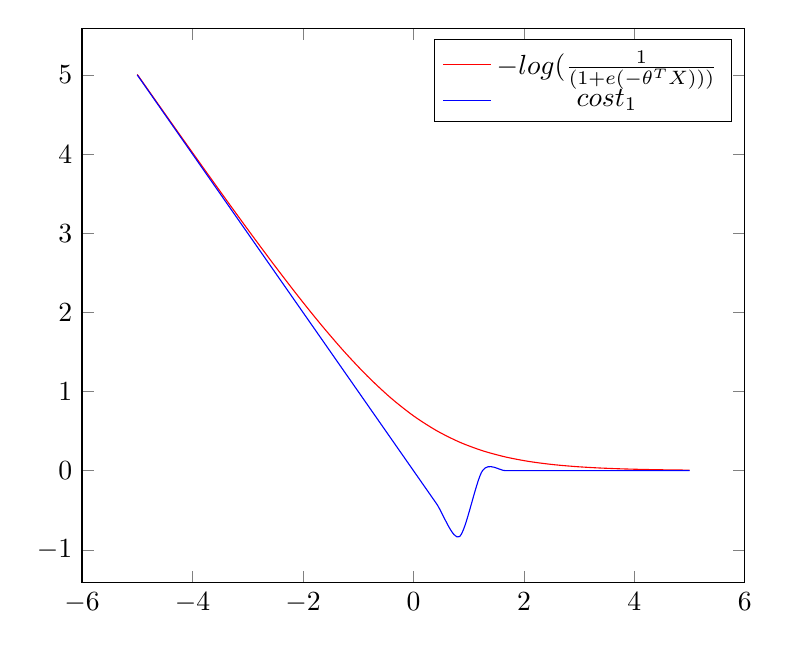
\begin{tikzpicture}
    \begin{axis}
      %TODO fix this graph!!
      \addplot[red,smooth] {-ln(1/(1+exp(-x)))};
      \addlegendentry{$-log(\frac{1}{(1+e(-\theta^TX)))}$}
      \addplot[blue, smooth] {(\x<=1) * (\x*-1) };
      \addlegendentry{$cost_1$}
    \end{axis}
  \end{tikzpicture}
    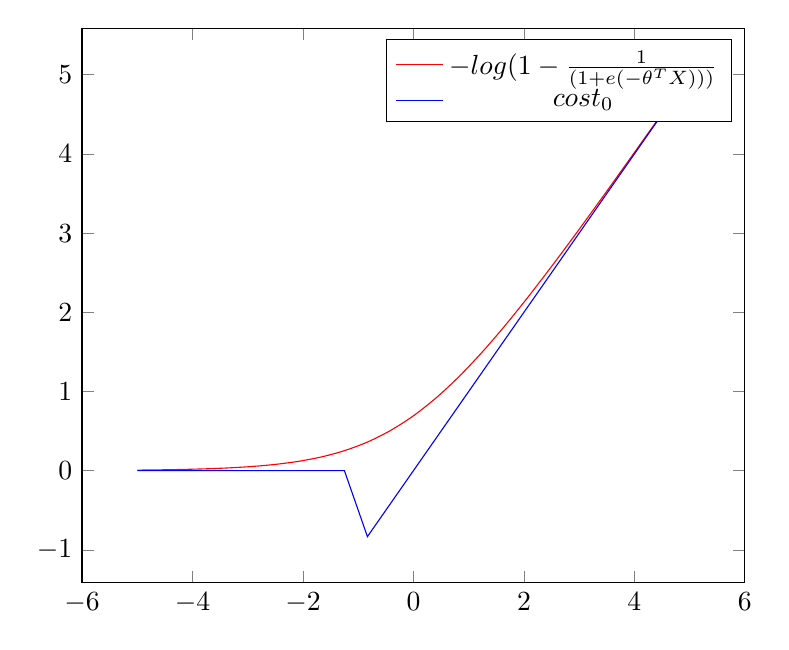
\begin{tikzpicture}
      \begin{axis}
        %TODO fix this graph!!
      \addplot[red,smooth] {-ln(1-1/(1+exp(-x)))};
      \addlegendentry{$-log(1- \frac{1}{(1+e(-\theta^TX)))}$}
      \addplot[blue] {(\x>=-1) * (\x*1) };
      \addlegendentry{$cost_0$}
    \end{axis}
    \end{tikzpicture}
%%
  \item $cost_1$: the linear lower bound of $-log(\text( h_{\theta})(x^{(i)})$ term, when y=1, and $\theta^TX>=1$
  \item $cost_0$: the linear lower bound of $-log(1-h_{\theta}(x^{(i)})))$ term, when y=0, and $\theta^TX<=-1$
  \item penalization term $\lambda$ is added to the first term instead,  $C \approx \frac{1}{\lambda}$, and finally, and averaging by m can be ignored since we multiply by large value C, and can also be ignored from the regularization term, since the $\theta$ is adjusted in the first term, note that the regularization term is just the Euclidean norm $\lVert \theta \rVert_2$
  \item the final SVM: $$C\sum_{i=1}^m[y^{(i)}(cost_1(\theta^TX^{(i)})) + (1-y^{(i)}) (cost_0(\theta^TX^{(i)})] + \frac{1}{2} \lVert \theta \rVert_2$$
  \item and the intuition for this is the first term get trained such that when $y=1$ then $cost_1=0$, if $y=0$, then $cost_0=0$, thus the first term is set to zero, and then SVM thrinks down to minimizing $$\frac{1}{2} \lVert \theta \rVert_2$$.
    \subsection{Large Margins in linear Decision Boundaries}
    \begin{description}
    \item it turns out that SVM do a pretty good job in decision boundary for given data-set, assume we classify class A against class B in the given data-set, first in a linear classification, it draw a line in between the two blobs of data, with nearly equal margins in both sides, the reason is in the hypothesis constrains $z=\theta^TX$, for $y=1$ then $z>=1$, and if $y=0$ then $z<=-1$, thus the model is trained to classify classes A,B outside the Large margin [-1\text{-}1], also note that the $\theta^Tx^i$ is the dot product (degree of alignment) between the weight parameter, and the training example $x^i$, and since z in required to be outside the defined range, thus z need to be a large value, meaning that both $\vec{x}$, $\vec{\theta}$ need to be aligned, otherwise z shrinks to zero at perpendicular angle $90^{\degree}$. if for example $\vec{\theta}$ is inclined w.r.t $\vec{x^{i}}$ by $\Theta^{\degree}$, then $\vec{\theta}$ need to be pretty large in order for z to lay outside ]-1\text{-}1[, but since we using penalizing factor $C$, then $\vec{\theta}$ is maintained to reasonable value, and thus the SVM model converges to the optimal decision boundary with large margins.
    \end{description}
    \subsection{Non-linear Decision Boundaries}
    \begin{description}
    \item previous hypothesis $\theta^TX$ is linear, in case of non-linear features, for example extracting faces for pictures, the problem is no longer classification of two categories, but rather features extraction of non-linear features from n-Dimensional example of n features. for example $ f(x) = \theta_1x_1 + \theta_2x_2+ \theta_3x_1^2 + \theta_4x_2^2 + \theta_5x_1x_2 + \theta_6x_1^2x_2^2 + \dots $ can be a good representative for capturing the non-linear boundaries for training example $x^i$ for all i in n. for a problem with large number of features is equation can be very expensive to train, instead choosing a appropriate polynomial of k-degree, to suits our problem decision boundary can be easier to train.
      \subsection{Gaussian kernel}
      \begin{description}
      \item in a non linear boundaries, where class A is surrounded by the class B scattered plots, the most appropriate used function is the normal, or Gaussian distribution function $$f(x)=\frac{1}{\sqrt{2\pi}\sigma}e^{-\frac{(x-\mu)^2}{2\sigma^2}}$$ yet instead of $\mu$ we use locality points (we will discuss this in the convolution neural network chapter), and since we deal with vector the numerator is the Euclidean distance $\lVert x^{(i)} - l^{(i)} \rVert$.
      \item so for each training example $x^{(i)}$ if it exists in the neighbourhood of the locality point $l^{(j)}$ for i,j $\in$ m. with computational cost $O(m^2)$ then f(x)=0, otherwise if the distance is too far, f(x)=1, thus SVM with Gaussian kernel hypothesis: $$C\sum_{i=1}^m[y^{(i)}(cost_1(\theta^Tf^{(i)})) + (1-y^{(i)}) (cost_0(\theta^Tf^{(i)})] + \frac{1}{2} \lVert \theta \rVert_2$$
      \end{description}
    \end{description}
  \end{description}
  \section{Unsupervised Learning (Introduction)}
  \begin{description}
  \item in \textbf{supervised learning}, given structure data-set of input X, and output Y, and the model has to be trained to map X $\rightarrow$ Y, in \textbf{unsupervised learning}, given only input X, the model has to be trained to extract similarities between input examples, thus classifying them into different coherent classes, for example in NLP, using clustering k-mean algorithm to compute word embedding similarity, or another more interesting example is identification of galaxies, and stars from astronomical pictures, another example is market segmentation, even when the data doesn't fit into separate coherent clusters, cut extend over a long range, it can be divided onto K number of classes/clusters
    \subsection{k-mean algorithm}
    \begin{description}
    \item given and input $X={x^1,x^2,\dots,x^m}$, randomly sample the K centroids (cluster centroids) over X, secondly is the assignment step, in which for each example $x^i$ for all i $\in$ m, $c^{(i)}$ is assigned  to the centroid with the shortest distance, thus taking the values $[1\text{-}k]$, so if $x^i$ is closest to $k^{\textbf{th}}$ then $c^{(i)}=k$, thirdly, and final step is the centroid movement, in which for each centroid $\mu_k$ for k $\in$ K, is relocated to the average of all points assigned to it.
    \item the cost function $$ J=1/m\sum_{i=0}^m\lVert x^{(i)} - \mu^{(i)} \rVert^2 $$
    \item to avoid falling into a local optima, multiple instantiation of the algorithm with different random initialization is advised, at the end the lowest cost is chosen.
    \item finally, if the number of clusters is unknown, and set arbitrary, then it need to commit to the constraint that $K <= m$, and whenever a centroid isn't assigned with any example, then K can be reduced by this number of unassigned centroids, or number of clusters can be plotted against the cost function, and we choose the pivotal k where the slop of cost changes significantly if any exist called \textbf{Elbow method}.
    \end{description}
    \subsection{Principle Component Analysis  PCA}
    \begin{description}
    \item another technique that will come useful later on in the NLP chapter is dimensionality reduction, having high-dimensional input data-set, with potentially redundant features, reducing the dimensions can be useful for both understanding data, and getting rid of redundancy, so for training data set with m training examples, of n features, let's assume that the input X $\in$ $R^{n}$ is projected into smaller subspace $R^{k}$, ignoring the bias feature term for simplicity.
    \item a straight forward algorithm is the Principle component Analysis, or PCA, for input features $X_{m\times{n}}$, $\Sigma=X^TX$ is the input for the single value decomposition SVD algorithm to de-factor it into $\textbf{U }\textbf{S }\textbf{V}$, for U being the Eigen vectors representing the n Dimensional space, and S is the Eigen values multiplied by $I_n$, in which the orthogonal matrices U, V have the property that any subset of U column for example first k columns denoted $U_k$ satisfy $U_k^TU_k=I_k$, therefore the projection into the k-Dimentional subspace spanning X is $U_kX$, or the projection of X on the subspace $U_k$.
    \item reduction shouldn't be done without losing much of the useful data, so it's wise to pick k, such that the lose of variance $<$ negligible value $\epsilon$, and can be estimated by the sum of the reduced eigen values, over the total sum in n dimension, so as to say $$\frac{\sum_{i=1}^kS_{ii}}{\sum_{i=1}^nS_{ii}} >= 1-\epsilon$$.

    \end{description}
  \end{description}

  \chapter{Structuring machine learning}
  \section{Machine learning strategy}
  \begin{description}
  \item we discussed in previous chapter how, and when to use optimization, regularization techniques, in practice, such decision making is crucial, and can save months of development time if we know to choose the right direction, and make the right decision to help our model work more effectively, doing regularization when the system need optimization in the case of high-bias is time consuming process, and spending months getting more data-set in highly biased model can be a total wast of time.
    \section{orthogonality}
  \item tuning process isn't done arbitrarily  but we must know which hyper-parameters to tune to get the most desired effect.
  \item modeling a process or a problem with as many features, we need to be able to fit our model to capture all data-set features. in the set of hyper-parameters it's easier if we can tune one parameter from the set of hyper-parameters and only take an effect on the corresponding purpose without avalanche effect, so for example in a car we can choose the adjust speed separately from the steering, although steering and speed are related in a single function, yet we can change one without affecting the other, therefor the name \textbf{orthogonality}
  \item doing well on training set, usually comparable to human level performance, depending on the application,... change the network into different architecture, use more efficient optimization algorithm i.e ADAM, etc
  \item doing well on the dev-set, in that order if the model is note fitting the dev set, meaning we have a high-variance, and we can use regularization, or getting a larger data-set.
  \item fit test-set well on the cost function, if we can't get our model to fit on the test-set in the other, then we probably over-tuned the model on the dev-set, and we need to re-tune with bigger dev-set.
  \item perform well in application, finally and in this order, if we can't capture the real application features in our model, then we then dev-test sets aren't quit fitting in the model, or we need to change the cost function.
    \section{Set up your Goal}
    \begin{description}
      \subsection{Evaluation metric}
      \subsection{Precision vs accuracy}
    \item accuracy/recall numerically the average of our prediction measurement is how var close to the reality.
    \item on the other hand, precision is how far our network prediction are True, or in other words is how far our predication are what they are.
    \item precision, and accuracy are orthogonal metrics, but there is a trad-off between both of them, in application, in the training process, it's advised to train different simultaneously (if possible) and plot their precision/accuracy metrics, and those the highest of all, getting high precision in one model, or high accuracy on the other, can't indicate which model is better.
      \subsection {F1-score}
    \item this metric is harmonic mean of precision \textbf{p}, and accuracy/recall \textbf{R}: $$\frac{2}{\frac{1}{P} + \frac{1}{R}}$$.
    \item with a single metric that combine how far our model is both accurate, and precise can be more efficient.
      \subsection {Satisfying-Optimizing metric}
      \item we might have a precise, and accurate model such as in case of F1-score, but yet it doesn't satisfy our practical application, in reality we are limited by time, and computational resources, and we need high \textbf{F1-score} relative to available resources, then a more general metric is a weighted average of F1-score, and our resource metrics, for example if we developing a network for recognition on phone we need the system to be both accurate/precise, but also to be under specific time threshold $T$, then our evaluation metric can be $F1-score*0.8+T*0.2$.
    \end{description}
    \section{train/dev/test sets}
    \begin{description}
    \item as discussed earlier in previous chapter that the ration of data-set partition into train, dev, and test sets are dependent on the data-set size, and the application really in accord with bias/variance scale.
    \item having a large enough training set can reduce variance, and sufficiently large enough dev set can enable us to have a deep perspective into the bias-variance scale, and finally the test set is essential to evaluate how var our low-bias, low-variance model fits on the same distribution of data.
      \subsection {dev/test metric}
    \item in case of very domain-specific training algorithm, for example a classification network on a very specific class $c_i$ or object out of the set of different classes C from our data-set of size n, we need to train our model to be aware of different classes, well distinguish between object rather than cat/not-cat binary classification, but also be able to classify our target object efficiently enough, we can add ad weighting parameter to the cost function evaluation: $$ J(w,b)=\frac{1}{\sum_{k=1}^{C_k}{w_k}} \sum_{i=1}^{m}w_k L(\hat{y},y) $$ where $w_k$ is the weight corresponding to each class $\begin{cases}w_1 \leftarrow \hat{y}=c_1\\w_2 \leftarrow \hat{y}=c_2\\...\\w_n \leftarrow \hat{y}=c_n\end{cases}$
    \end{description}
    \item it's important to note that if the distribution of the practical input-set is of different features than that of our train/dev/test distribution, our model can be guaranteed to do well in practice.
  \end{description}
  \section{Human-level performance}
  \begin{description}
  \item in the past few years machine learning have surpassed human cognitive levels in different areas, performance of machine today overshadow that of humans, in the past decades the accuracy of machine has been increasing linearly up to level slightly higher than the human's.
  \item as long as the machine level is lower from that of the humans we can boost it with human-labeled data, gain a better insight from error analysis, better analysis of bias/variance , as to increase it's cognitive abilities
    \subsection{human(bayes) error}
  \item as machine level rises high to humans, we can add another level the train/dev/test cycle, that is human level error, and interpretation from human/bayes level to training error is called the \textbf{avoidable bias} error, and difference in error between training and development is the \textbf{variance}.
  \item we can use avoidable bias, and variance as a metric for how well our model perform, and optimize our model, and network to reach human level performance, and minimize that error.
  \item comparing those two metrics tell us where to optimize, for example if the avoidable bias is 4%, and the variance error is 10% then it's wiser to resolve the over-fitting of the model before achieving human-level performance.
    \item the human level performance is really lose, comparable to how well our model is trained to achieve low variance error, humans as well difference in their levels of cognitive ability fitting a normal distribution naturally, but if an average human is to be compared to a guru in the specific domain, then the guru of sufficient skill-set, and training is able to achieve lower Bayes error, and the latter varies greatly, for example in radiology, an average human is expected to achieve higher error of diagnosis, and recognition  compared to skilled doctor, and the latter compared to a team of doctors, choosing specific human-level from the domain of human-cognition is another problem.
  \end{description}

  \section{Error analysis}
  \begin{description}
\item taking the right decisions in what to invest your time in while optimizing a model can be a great leverage and can save month, if not years of Engineering time! making error analysis is just one of those.

\item statistical analysis of the mismatched predictions $\hat{y}$ at the test time cat is coined the name \textbf{Error analysis}.
\item Assume for example that error analysis taking from the sample of mismatched predictions shows that false-negative is 50\% percent, then it would be wise to spend time enhancing our model for predictions, and cut down the ratio of 50\% to a reasonable ratio, perhaps 2\% .
\item for example in a classifier network, out of N mismatched predictions are actually what we expect (of being a specific class), but the model classified otherwise, from the N mismatched predictions we take for example 100 entry, and analyse the false-negatives. if it shows that the ratio is 50\% for example then we are on the right track to regard this as bias problem, and invest time on it, on the other-hand if out of the 100 entries only 3\% were false-negatives then, it's not our priority to invest time down this road, and to achieve such high accuracy is actually indication that we might not be able to do better, and it's more wise to move on, and spend time optimizing our model to get a low false-negatives on other classes from our error analysis, or train our model on certain features that might be mis-classified.
  \subsection{Mislabeled  data}
\item another perspective to Error analysis is to record the mislabeled input data, it turns out that deep learning is quite robust against small randomly mislabeled data, so in big data of millions of entries, if the mislabeled data are randomly distributed over the data-set classes, and it's a below acceptable error, it's really unwise to spend months fixed mislabeled data since deep learning prove to be robust against just errors.
\item so far there are three metrics in error analysis to consider, first the overall false-negatives, we take this ration, and sum the ratio of each prediction, thirdly the ratio of mislabeled data, comparing the three metrics can give us insight to help enhance our model, and reduce the overall error, if the overall error is reduced, meaning our model accuracy is acceptable compared to human level, we still have two metrics, to choose from, if the prediction-error (overall-error - mislabeled-error) from the dev-set is reduced after we choose between models, and the test error is also reduced then it can be wise to spend time on mislabeled input data.

  \section{Mismatched training dev/test sets}
  \begin{description}
  \item it turns out in practice the model's input usually tend to noisier than the training/dev/test sets input, which are filtered for example in computer vision, input data-set can be of a common distribution of high-resolution, close proximity, centered object, while user input can be blurry, of low-resolution, or in speech recognition we train our model on a clear audio, yet in practice there will be stutter, background noise, etc.
  \item there is a trade-off between choosing data-input between different distribution, and accuracy, and choosing data from different distribution can really help but under the following criteria, that the dev/test phases need to aim at our target, meaning to be chosen completely from target data, while the training data-set can be a shuffle of different distributions.
  \item in this scenario new error is introduces, consider that the training error is 1\% and the dev error is 10\% then it's possible to tell wither our model is over-fitting or it's result of mismatch data from different distribution?! to help make a decision, the data-set is divided into training/train-dev/dev/test sets, where train-dev, and training sets are form the same shuffled distributions, while dev/test sets are of our target data, so addressing the same problem if the train error is 1\%, and the train-dev error is 9.5\%, while the dev error is 10\% then it's a variance problem, but if the train-dev error is 1.5\%, and the development error is 10\% then our model is getting mismatched data.
  \item lastly, and as previously discussed if the test error say 15\% then our test set of the same target distribution as the dev-set is over-fitting the dev-set, and to fix this, we ought to increase the dev-set.
    \subsection{Addressing data mismatch}
  \item in case of data mismatch in a shuffle of distributions, or in other words the wide error difference between train-dev set, and the dev set, this is an indication of the gap between the data-sets from different distributions.
  \item a close examination of that difference through error analysis help taking the right decision to reduce this difference, and choosing training data from distribution closer to the target data.
    \subsection{Artificial data synthesis}
  \item if the target data-set is limited as usual in practice, given a target data set of size m, it's possible through artificial data synthesis techniques to increase this size to 100m, or even as large as 1000m, but in this case it's possible to run into an over-fitting problem if the original m data set isn't representative enough.
  \end{description}

  \section{Multiple tasks learning}
  \begin{description}
    \subsection{Transfer learning}
    \item when we train a model in a very domain-specific application with very limited data-set, we can employ weight-transfer, also known as transfer learning, and pick the closest general domain to our domains-specific application, and randomly initialize the last layer's weight $w^{[L]}$, leaving the rest of weight as they are, and through the new domain-specific data set $(X,Y)$ old $w^{[l]}$ $ | l \in [0-L[$, and randomly initialized $w^{[L]}$ we can scale the old model to the new model very quickly.
    \end{description}
    \subsection{Multitask learning}
    \item in transfer learning we make use of previously trained weights to train our model on a newly different task usually in cases when there isn't sufficient data of the second class, but in cases when there is a need to extract as many features from the same example, and the same model, previously we discussed softmax activation function for training a model for multi-class classification, but in different cases of multitasking models rather than multi-class model, for example in object detection in a video, we need to extract boundaries around n set of object $\{o_1,o_2,...,o_n\}$ with bounding box surrounding each object, compared to multi-class problem then we just satisfied with the prediction of $\hat{y}$ in a sparse hot-vector, but in the multitask the label $Y$ is vector with more than a single entry of each task, in this we employ what is called Multitask learning, in the following chapter we will deal such case.
  \end{description}

  \section{End-to-End Machine Learning}
  \begin{description}
  \item .
  \end{description}

  \chapter{Computer Vision}
  \section {Object Detection}
  \begin{description}
  \item In previous chapters we discussed classification neural networks, for a given input $x_i$, being an image, and prediction (estimate) $y$ is the classification wither in a binary representation 0/1 of size 1, or on-hot vector of multi-class classification, in case the input contains more than one class, known as multi-tasking. so far
  \item classification in computer vision is one of the building blocks, feeding input $x_i$ to the NN, and getting an estimate of the classes inside the pictures isn't sufficient, when we (humans!) look at a picture we first locate the objects, then classify each of them, then derive a meaning. in computer vision we focus on the first two steps.
  \item object detection is about How to locate all the objects in the picture simultaneously? but before that, in previous chapter we discussed that it's advised to use min-batch in the case of large NN compared to the available computational power, and memory, having a moderate resolution picture as an input i.e $1024 \times 1024$ of 3 channels, if the first layer consist of just 1000 neurons we end up with billions of parameters to train! with huge amount of parameters, and features to capture, if we doesn't have sufficient data-set, then our model will be over-fitting the data-set, then how to solve it?
  \item convolution solves this problem, it makes use of the \textbf{sparsity of connections} (in each layer, each output value depends only on a small number of inputs), and \textbf{parameter sharing} (that a single features detector or a filter is shared between features) and we will discuss it in the following sections.
 \item due to sparsity of connection convolutions NN good at capturing translation invariance, meaning a network is capable of getting the same output of a slightly shifted image, we will see why.
   \subsection{Edge Detection}
   \begin{description}
    \item for input image $x_i$ how to detect the boundaries? how to interpret it mathematically?
    \item first, edge boundaries of $2\times2$, or $4\times4$ pixels can be vertical, horizontal, or inclined by $n^{\circ}$, to extract such features of image $g(x)$ by filter $f(y)$, is a process of weighting image \textbf{g} by the filter \textbf{f}, or mathematically, it's the integral of all the shifts in shifted, and reversed function g, or f $$ \int_{\infty}^{-\infty}{f(\tau)*g(x-\tau)d\tau} $$ (see the appendix on convolutions)
    \item to detect a vertical edges a vertical edge detection can be as simple as $\begin{bmatrix}1&0&-1\\1&0&-1\\1&0&-1\end{bmatrix}$, or with more emphases on the center.
    \item for example to detect horizonal edges, we employ
      $f(\tau)=\begin{bmatrix}
      1&1&1\\
      0&0&0\\
      -1&-1&-1\end{bmatrix}$, for image $g(x)=\begin{bmatrix}
      10&10&10&0&0&0\\
      10&10&10&0&0&0\\
      10&10&10&0&0&0\\
      0&0&0&10&10&10\\
      0&0&0&10&10&10\\
      0&0&0&10&10&10\end{bmatrix}$ then convoluted
      $\int_{\infty}^{-\infty}{f(\tau)*g(x-\tau)d\tau}$ evaluated to $\begin{bmatrix}
        0&0&0&0\\
        30&10&-10&-30\\
        30&10&-10&-30\\
        0&0&0&0 \end{bmatrix}$
      \item more filter examples: \begin{itemize}
      \item \textbf{sobel's filter} is $\begin{bmatrix} 1&0&-1\\ 2&0&-2\\ 1&0&-1\end{bmatrix}$.
      \item identity filter function $\begin{bmatrix}
        \ \ 0 &\ \  0 &\ \  0 \\
        \ \ 0 &\ \  1 &\ \  0 \\
        \ \ 0 &\ \  0 &\ \  0 \end{bmatrix}$
      \item  another sharper edge detection filter $\begin{bmatrix}
        -1 &  -1 & -1 \\
        -1 & \ \ 8 & -1 \\
        -1 &  -1 & -1 \end{bmatrix}$
      \item sharpen filter $\begin{bmatrix}
        \ \ 0 & -1 & \ \ 0 \\
        -1 & \ \ 5 & -1 \\
        \ \ 0 & -1 & \ \ 0
      \end{bmatrix} $
      \item blur box filter $\frac{1}{9}
        \begin{bmatrix}
          \ \ 1 &\ \  1 &\ \  1 \\
          \ \ 1 &\ \  1 &\ \  1 \\
          \ \ 1 &\ \  1 &\ \  1
        \end{bmatrix}$
      \item Gaussian blur filter $\frac{1}{16}
        \begin{bmatrix}
          \ \ 1 &\ \  2 &\ \  1 \\
          \ \ 2 &\ \  4 &\ \  2 \\
          \ \ 1 &\ \  2 &\ \  1
        \end{bmatrix}$
      \item larger $5\times5$ Gaussian blur filter $\frac{1}{256} \begin{bmatrix}
        1 & 4 & 6 & 4 & 1 \\
        4 & 16 & 24 & 16 & 4 \\
        6 & 24 & 36 & 24 & 6 \\
        4 & 16 & 24 & 16 & 4 \\
        1 & 4 & 6 & 4 & 1
      \end{bmatrix}$.
      \end{itemize}
        \subsection{Padding}
      \item from previous example you can notice that $6\times6$ input image was shrunk into $4\times4$ matrix (\textbf{known as valid convolution}), also the boundary edges are dismissed, to maintain the same output size to the input size (\textbf{known as the same convolution}) we use padding:
      \item for input image of size $n\times n$, and filter of size $f\times f$, the output is $n-f+1\times n-f+1$, for same convolution we pad the edges with p cells, such that $p=f-1/2$ then final output image size $n+2p-f+1\times n+2p-f+1$, for this equation to hold, then filter size have to be \textbf{odd}, and it's usually the case in computer vision, look at the \textbf{identity filter}, where the weighting parameters are set to zero, while the \textbf{center pixel} is set to 1.
      \item to pad our previous  examples we get the following image with $p=1$ $g(x)=\begin{bmatrix}
        0&0&0&0&0&0&0&0 \\
        0&10&10&10&0&0&0&0\\
        0&10&10&10&0&0&0&0\\
        0&10&10&10&0&0&0&0\\
        0&0&0&0&10&10&10&0\\
        0&0&0&0&10&10&10&0\\
        0&0&0&0&10&10&10&0\\
        0&0&0&0&0&0&0&0\end{bmatrix}$
        \subsection{striding}
        \item ?
    \end{description}
    \subsection{Convolution on RGB channels}
    \begin{description}
      \item In 3 RGB channels $n_c=3$, on image $n\times{n}$ we add filter for each channel $f\times{f}\times{n_c}$, and the output image is $n-f+1 \times{n-f+1} \times{1}$
    \end{description}
    \subsection{Multiple filters Convolution}
    \begin{description}
      \item for layer $L$ of size $n\times{n}\times{n_c}$, there is always more than a single features, and therefore requires filter for each feature, so filtering layer end up being $f\times{f}\times{n_c}\times{n^*}$ such that $n^*$ is the number of filters for layers, and the output is $n-f+1\times{n-f+1}\times{n^*}$.
    \end{description}
    %\subsections{Notations}
    \subsection{Example ConvNet}
    \begin{description}
    \item in case of input image $n_H^{[0]}=n_W^{[0]}=39, n_c^{[0]}=3$ of size $39 \times{39} \times{3}$, using 10 filter of size $f^{[1]}=3$, and strides $S^{[1]}=1$, padding $P^{[1]}=0$ and 10 filters, then layer 1 will deterministically be of a size  $\left \lfloor{\frac{n^{[1]}+2p^{[1]}-f^{[1]}}{s^{[1]}}}\right \rfloor + 1=37$, then $n_H^{[1]}=n_W^{[1]}=37,n_c^{[1]}=10$.
    \item in layer 2, using 20 filter of size $f^{[2]}=5$, and strides $S^{[2]}=2$, padding $P^{[2]}=0$, then layer 2 will deterministically be of a size  $\left \lfloor{\frac{n^{[2]}+2p^{[2]}-f^{[2]}}{s^{[2]}}}\right \rfloor + 1=17$, then $n_H^{[1]}=n_W^{[1]}=17,n_c^{[1]}=20$.
    \item in layer 3, using 40 filters,  of size of size $f^{[3]}=5$, and strides $S^{[3]}=2$, padding $P^{[3]}=0$, then layer 3 will deterministically be of a size  $\left \lfloor{\frac{n^{[3]}+2p^{[3]}-f^{[3]}}{s^{[3]}}}\right \rfloor + 1=7$, then $n_H^{[1]}=n_W^{[1]}=7 ,n_c^{[1]}=40$.
    \item flatten layer3 $7 \times{7} \times{40}$ into $1960\times{1}$ and activate it through softmax/logistic function, where last layer 5 is $1\times{1}$.

    \end{description}
    \subsection{Pooling Convolutions}
    \begin{description}
    \item along side convolution NN, there Pooling layers are used to make the network more robust, and cut down the size of parameters.
    \item most used parameters are $f=2,s=2$, or $f=3,s=2$, and padding is rarely used.
    \item note that there is no learned parameters in pooling, so max-pooling layer doesn't count as a stand alone layer since no parameters to train, and rather seen as part of the layer operating on.
      \subsection{Max Pooling}
      \begin{description}
      \item pooling is $n\times{n}$ layer, and services to divide the input layer into smaller $n\times{n}$ layers and leaving only the maximum value of which it's an \textbf{argmax} convolution function, the convolution function takes the argmax instead o the integral.
      \item for example, input layer $\begin{bmatrix}1&3&2&1\\2&9&1&1\\1&3&2&3\\5&6&1&2\end{bmatrix}$, with $strides=2$, convoluted by $2\times{2}$ max-pooling into $\begin{bmatrix}9&2\\6&3\end{bmatrix}$
      \end{description}

      \subsection{Average Pooling}
      \begin{description}
      \item similar to max pooling except argamx is replaced with the mean function.
      \item for example, input layer $\begin{bmatrix}1&3&2&1\\2&9&1&1\\1&3&2&3\\5&6&1&2\end{bmatrix}$, with $strides=2$, convoluted by $2\times{2}$, max-pooling into $\begin{bmatrix}3.75&1.25\\4&2\end{bmatrix}$.
      \end{description}
    \end{description}
    \section{Examples}

      \subsection{LeNet-5 Network}
      \begin{enumerate}
      \item Layer 0: with input image $n_H^{[0]}=n_W^{[0]}=32$, $n_c^{[0]}=3$.
    \item Layer 1: using 8 filters, $f^{[1]}=5$, $s^{[1]}=1$, we get $28 \times{28} \times{8}$, adding  max-pooling with $f=2, s=2$, pours down into $14\times{14}\times{8}$ layer.
    \item Layer 2: using 16 filters $f^{[2]}=5$, $s^{[2]}=1$, we get $10 \times{10} \times{16}$, adding  max-pooling with $f=2, s=2$, pours down into $5\times{5}\times{16}$ layer, flattened into $400\times{1} vector$
    \item Layer 3: Fully-Connected (FC3) layer of 120 neurons, with weight, bias parameters $W^{[3]}, b^{[3]}$.
    \item Layer 4: FC4 layer of 84 neurons, and $W^{[4]},b^{[4]}$, feed to softmax activation with 10 neurons output.
      \end{enumerate}
    \item notice the size of parameters in convolution layers compared tota \textbf{FC} layers, in \textbf{CONV1}, \textbf{CONV2} number of parameters are 208, 416 respectively compared to 48001, 10,081 in \textbf{FC3}, \textbf{FC4} respectively. meanwhile the \textbf{Activation size} falls down gradually, from 3.072 the number of pixels in the image to 10 neurons in the softmax classification, and 6.272, 1.568, 1.600, 400, 120, 84 in CONV1, POOL1, CONV2, POOL2, FC3, FC4 respectively.
  \end{description}
  \subsection{AlexNet Network}
  \begin{enumerate}
  \item Layer 0: input is $227\times{227} \times{3}$,
  \item Layer 1: applying 96 filter with size 11, and stride=4, the output is $5 \times{5} \times{96}$ max pooled by $3\times{3}$ of strides of size 2, the input is $27\times 27 \times 96$.
  \item Layer 2: applying 256 filter, of \textbf{SAME} padding, of size 5, outputs $27 \times27 \times 256$, max-pooled by size 3, and stride size=2 outputs $13 \times 13 \times 256$.
  \item Layer 3: 384 filters with SAME padding convolutions, outputs $13 \times {13} \times {384}$.
  \item Layer 4: 256 filters with SAME padding, outputs $13\times{13}\times{256}$ max-pooled by size 3, and strides of size 2, outputs $6\times{6}\times{256}$ flattened into $9216\times{1}$.
  \item Layer 5: fully-connected $4096\times{1}$, by $4096\times{1}$, then softmax of 1000 neurons/predictions.
  \item compare the two networks, LeNet-5 from the nineties with around 60000 parameter, to 2012 AlexNet with 60 million parameters, despite this, they are similar in structure.
  \end{enumerate}


  \subsection{VGG-16 Network}
  \begin{description}
  \item VGG similar AlexNet, yet deeper, with narrower convolution proven to be more powerful.
  \item using [CONV] of size $3\times{3}$, strides size=1, of SAME padding, MAX-POOLing of size $2\times{2}$, with strides size=2.
  \item consist of 16 layers therefore the name VGG-16, with ~138Million of parameters, and it's network is:  $[CONV64\times{2}] \rightarrow [CONV256\times{3}] \rightarrow [CONV512\times{3}] \rightarrow [CONV512\times{3}] \rightarrow [FC4096] \rightarrow [FC4096] \rightarrow [SOFTMAX1000]$
    \end{description}
  \begin{enumerate}
  \item  $224\times{224}\times{3}$ input image.
  \item  applying $[CONV64] \times{2}$, (convolutions of 64 filters twice), outputs $224\times{224}\times{3}$. [MAX-POOL]ed into $112\times{112}\times{64}$
  \item  $[CONV128]\times{2}$ [MAX-POOL]ed into $56\times{56}\times{128}$.
  \item  $[CONV256]\times{3}$ [MAX-POOL]ed into $28\times{28}\times{256}$
  \item  $[CONV512]\times{3}$ [MAX-POOL]ed into $28\times{28}\times{512}$
  \item  $[CONV512]\times{3}$ [MAX-POOL]ed into $7\times{7}\times{512}$
  \item $[FC4096]$ fully connected layer with  4096 nodes
  \item $[FC4096]$ fully connected layer with  4096 nodes
  \item $[SOFTMAX1000]$  softmax activation with 1000 entries.
  \end{enumerate}
  \subsection{ResNet (Residual Block)}
  \begin{description}
    \item Very deep network are much difficult to train because of vanishing, and exploding gradients, to make this feasible,  \textbf{Residual blocks} was introduced
    \item even with the use of an Optimizer to lessen the vanishing/exploding gradients, in a very deep network with hundreds or even thousands of layers, which are rarely used, the number adds up, and either diminishes to zero, or explode into large numbers. residual blocks adds the activation from a previous layer (i.e $l-2) $into the current activation function $l$, $a^{[l]}=g(z^{[l]}+a^{[l-2]})$, also known as \textbf{shortcut}, or \textbf{skip connection}.
    \item assume for example we using regularization and $w^{[l]},b^{[l]}\rightarrow{0}$, then $a^{[l]}=g(a^{[l-2]}$, residual would prevent vanishing gradient.
    \item note that skip connection between $a^{[i+n]}$, and $a^{[i]}$ for $i,n \in N$, can be between two different sizes, in practice same padding is used between shorted layers, or through function W, such that shape of $a^{[i+n]}=W.a^{[i]}$. that can for example zero pad the ith layer.
      \item .
  \end{description}
  \section{Inception}
  \begin{description}
  \item another parameter to worry about is the size of convolution kernel, instead of testing out different sizes, it's possible to combine all of them at once with SAME padding, and let the model train, and figure out the most convenient of all, called \textbf{Inception network}, on a computational cost.
  \item for example in input network of size $28\times{28}\times{192}$, we can combine $1\times{1}$, $3\times{3}$ SAME padding, $5\times{5}$ SAME padding, and MAX-POOLing SAME padding, to get $28\times{28}\times{256}$ network. in this example note that the computational cost is for 120 million parameter.
    \subsection{$1\times{1}$ Convolutions}
    \begin{description}
    \item in such very expensive layer, what we can do to reduce the computational cost is convolution of $1\times{1}$ times the factor or reduction, for example in the previous example we can pick fittest filter through [CONV1], with 16 kernel, applying second [CONV5] with 32 filters we end up with $28\times{28}\times{32}$ layer, so we manage to pick the fittest kernel, and also reduce the computation cost for 120 million parameter to just 12.4 million.
      \item
    \end{description}
    \subsection{Inception Block}
    \begin{description}
    \item the inception network is a series of block of the following building block: (insert the szegedy paper picture here)
    \end{description}
    \subsection{Inception Branches}
    \item (insert the szegedy paper picture here)
      \section{Object Detection}
      \subsection{Localization and Detection}
      \begin{description}
      \item  in computer vision network the output layer is usually a vector of localized objects rather than an one-hot vector representing a specific class, and the process is divided into three steps, first \textbf{Detection}, second \textbf{Localization}, lastly \textbf{classification}.
        \subsection{classification with localization}
      \item  one-hot vector SOFTMAX output can be combined with localization, to locate, specific target class in an image, boxing our target object with $b_w\times {b_h}$ with Cartesian coordinates of the image center $(b_x,b_y)$, now three are 4 more parameters. $b_x, b_y,b_w, b_h$ for localization.
      \item labeled output vector with localization: $$\begin{vmatrix}p_c | \text{a Boolean for wither there is an object or not}\\
        b_x\\b_y\\b_h\\b_w\\c_1 | \text{first class}\\c_2 \text{class 2}\\...\\c_n | \text{class n}\end{vmatrix}$$. if $p_c=0$ then the rest of the vector's elements will be zero.
      \item Loss function $L(\hat{y},y)$ will be element wise operation. but practically different loss functions can be used on different ranges of  $y$ for example log-likelihood on range [$c_1$-$c_n$], and mean squared on the bounding box coordinates range, and logistic regression loss.
      \end{description}
      \subsection{Landmark detection}
      \begin{description}
      \item it's possible to go deeper beyond the bounding box, and train model on labeled data-set with desired landmarks on the target object, for example after along side localization of the humane face with bounding box, it's possible to add landmark features for example to locate the human mouth, eye's, and cheek boundaries, so to extract the facial expressions, another example could be tracking the skeleton, and joints for pose estimation of an athlete during exercise, also used in augmented reality applications.
      \item to place 50 landmark on a single object to locate it's boundaries with two Cartesian coordinates points means extra 100 entry inside the labeled data-set entries.
      \end{description}
      \subsection{Object Detection}
      \begin{description}
      \item to detect, locate objects in input image of size $N\times{N}$.
      \item run sliding window cropping function over input image cropping images with re-sizable starting with length = l, with certain strides.
      \item sequencially iterate through the previous step increasing the length l for larger crops, this is a problem with $O(N^2)$ computational complexity.
      \item then final step is to run the cropped images in the classifier.
        \subsection{Convolutional sliding windows}
        \begin{description}
        \item sliding window cropping is computationally expensive, if you have noticed that for every crop, the model expected to forward the cropped image to be classified, then increasing the complexity by the number of crops.
        \item the shared parameters characteristic of the convolutions can a great leverage to solve this problem, and cut the complexity significantly, by running the whole iterations simultaneously, it can be illustrated by an example.
          \subsection{Example:}
          \begin{description}
          \item for the following network classifying input image(expected input) of size $14\times{14}\times{3}$, $[CONV5]\rightarrow [MAX-POOL2-5] \rightarrow [FC5-400] \rightarrow [FC1-400] \rightarrow [SOFT-MAX-4]$. with the corresponding size $10\times{10}\times{16}\rightarrow 5\times{5}\times{16} \rightarrow 1\times{1}\times{400} \rightarrow 1\times{1}\times{400} \rightarrow 1\times{1}\times{4}$ we end up with 4 neurons (softmax output) being our classification model, for an input image  with size $28\times{28}\times{3}$ and sliding window $14\times{14}$ to fit in our model, running the same convolution network above on this input  $[CONV5]\rightarrow [MAX-POOL2-5] \rightarrow [FC5-400] \rightarrow [FC1-400] \rightarrow [SOFT-MAX-4]$. with the corresponding size $24\times{24}\times{16}\rightarrow 12\times{12}\times{16} \rightarrow 8\times{8}\times{400} \rightarrow 8\times{8}\times{400} \rightarrow 8\times{8}\times{4}$ such that the most upper right cell $1\times{1}\times{4}$ of coordinates (0,0) is actually corresponding to the simplified model output above, and the second (0,1) output is one slide to the right, and so on.

          \end{description}

        \end{description}
      \end{description}
      \section{Bounding Box prediction}
    \item the aspect ratio of the bounding box isn't really fixed, and to wrap the detected object correctly, then there are two variables in the sliding box instead of one in sequential terms.
        \subsection{YOLO}
        \begin{description}
        \item YOLO is a convolutional network, but we can explain it from a sequential iterative perspective that the input image is divided up into $k\times{k}$ cells, running the sliding window function in each cell, then simultaneously, so instead of getting a single $8\times{1}$ output, we get $k\times{k}\times{8}$ output, the localization algorithms runs in a single cell.
        \item even if the object stretches on multiple grid cells, it's only assigned to a single cell.
        \item to specify the bounding box inside a grid, the center of the detected object is coordinated with respect to the origin(0,0) of the cell on the top most left, and the bottom right assigned to (1,1), therefore the center$(b_x,b_y)$ must be between 0,1, where as the $b_w,b_h$ can be greater than 1 if it wraps multiple cells, and it's measured by the ratio with respect to the cell width, or height respectively.
        \end{description}
        \subsection{Jaccard distance, or Intersection over Union IOU function}
        \begin{description}
          \item it's an accuracy metric for how well the model is performing, and defined by the area of intersection between the prediction, and the labeled bounding boxes, over the prediction area. indicating how far this predicted bounding box fits into the ground truth table.
        \end{description}
        \subsection{Non-Max Suppression}
        \begin{description}
        \item in practice the input image is divided up into very fine cells, and a single object can overlap multiple cells, Non-Max suppression is algorithm to choose the maximum overlapping cell, and assign the detection with is, suppressing other cells, therefore the name.
        \item the metric for overlap is the $p_c$ in the output layer, previously we assigned $p_c$ to either 0, or 1, but in this case is the probability of overlap, and only the highest bounding box's $p_c$ remains, suppressing the rest.
        \end{description}
        \subsection{Anchor Boxes}
        \begin{description}
        \item in a single cell there could coexist more than one object, we expect multiple object each with specific aspect ratio, then we consider more than sliding window also known as \textbf{Anchor Box}, each with different aspect ratio, and the output $y,\hat{y}$ will look like the following for m anchor boxes but flattened into a single vector $$ \begin{vmatrix}p_c^1&p_c^{2}&...&p_c^{m}\\p_x^{1}&p_x^{2}&...&p_x^{m}\\p_y^{1}&p_y^{2}&...&p_y^{m}\\p_h^{1}&p_h^{2}&...&p_h^{m}\\p_w^{1}&p_w^2&...&p_w^{m}\\c_1^{1}&c_1^{2}&...&c_1^{m}\\...\\c_n^{1}&c_n^{2}&...&c_n^{m}\end{vmatrix}$$
        \end{description}
        \subsection{Region Proposal R-CNN, Fast R-CNN}
        \begin{description}
        \item instead of running the sliding window on everywhere in all cells, with the same slide, it can be more appropriate to narrow this down into very specific regions: first the input image is run through semantic segmentation function, dividing up the input into blobs(Regions proposal), then the Anchor boxes are run on top of them, but this process turns out to be very slow.
        \item Fast R-CNN is a convolution implemtnation of it, and speeds up the process a bit.
          \end{description}
        \item .
  \end{description}
  \section {Face Recognition }
  \subsection{Recognition vs. Verification}
  \begin{description}
  \item in verification given an input image, name/ID, verify whether the input image is that of the claimed person, on the other hand, in a databaseof K persons, given an image, Recognize the image to one of the images in the database.
  \item having 99\% accuracy in the verification process is good enough threshold, meanwhile in recognition in database of 1000 persons, having 99\% accuracy means that the classifier works with uncertainty  of 1 to 10, there our classification model maps the image to 10 out of 1000 with equally likely probability, so accuracy in recognition need to  approach 100 percent.
  \end{description}
  \subsection{One-Shot learning}
  \begin{description}
  \item addressing the following criteria given a single input image for a person, as a single entry in the training-set, our model need to have accuracy approaching 100\%. for new inputs to the trained model, how to scale?
    \subsection{Similarity learning function}
    \begin{description}
    \item given two images $I_1,I_2$, then similarity function $d(I_1,I_2)$ calculates the distance, and the distance inverse is how identical the two images are, such that $d=0$ if $I_1=I_2$, and verification is acceptable under negligible distance threshold $\tau$: $$
      \begin{cases}
        same  \leftarrow d(I_1,I_2) \leq \tau \\
        different \leftarrow d(I_1,I_2) > \tau
      \end{cases}
      $$
      \item a convolution example is the Siasmese network:
    \end{description}
    \subsection{Siamese Network}
  \item how to calculate the similarity distance?
    \begin{description}
    \item for an convolution network ending with fully-connected with N nodes [FCN] layer, then for each data-set entry $x^{(i)}$, we define $f(x^{(i)})$ to be the output of [FCN] on the entry $x^{(i)}$.
    \item for two input images $x^i, x^j$ from the data-set, the similarity function: $$ \|f(x^{(i)}) - f(x^{(j)})\|_2^2 $$.
    \item so, how to define the loss function? using what is called a \textbf{Triplet Loss}
      \subsection{Triplet Loss}
      \begin{description}
      \item Loss function is defined on top of the similarity function d, in terms of  distance between current image $x^i$, and the whole data-set images, the model can be trained on a single image called \textbf{Negative} $x_i^{n}$ with large distance, and \textbf{Positive} $x_i^{n}$ image with small distance, against the current image called \textbf{Anchor image} $x_i^{a}$, and the loss function for the triplet can be defined as $L(d(x_i^a,x_i^p), d(x_i^a,x_i^p))$.
      \item but to prevent against the trivial solutions for triplets of the same persons, a marginal $\alpha$ is used, so the final loss equation is for N triplets: $$
         \sum_i^N {\|f(x_i^a) - f(x_i^p)\|_2^2  - \|f(x_i^a) - f(x_i^n)\|_2^2} + \alpha
        $$
      \end{description}
    \item  what to do in case of new input images?!
      \subsection{Binary Classification}
      \begin{description}
      \item another variation is binary classification into ``match'', or ``not match'', can be performed into pair of images $x^i, x^j$, and label 0 (for different persons), or 1(for the same person), with Sigmoid activation, defined as of [FC] layer of size F: $$
        \hat{y}=\sigma (\sum_k^{F} w_i \|f(x^{i})_k - f(x^{j})_k \| + b)
        $$ where $w_i, b_i$ are training parameters.
      \item or using the qui-square formula $$
        \frac{(f(x^i)_k - f(x^j)_k)^2}{(f(x^i)_k + f(x^j)_k}
        $$
        \end{description}
    \end{description}
    \section{Neural Style Transfer}
    \begin{description}
      \item first of all how to define style? style is the variations, or shades of specific content, and inside the neural network style transfer can be length of correlation between activations across different channels.
      \item artistic style transfer, is the transfer of style of the Style image \textbf{S}, to the content image \textbf{C}, that outputs the generated image \textbf{G}.
      \item cost function can be defined on the generated G, as follows: $$J(G) = \alpha J_{content}(C,G) + \beta J_{style}(S,G) $$ using weighting parameters $\alpha, \beta $ to control how far the generated image is closer to either the content, or the style (note that a single weight is sufficient, for example $\alpha, and (1-\alpha))$ minimizing the cost between both the style, and the generated image, and the content, and the generated, thus merging the content, and the style images.
        \subsection{Generated image descent}
        \begin{description}
      \item gradient descent is minimizing J(G), rather than weight parameters. $$ G=G-\frac{\partial{J(G)}}{\partial{G}} $$
      \item the final generated image descent is as simple as: \begin{enumerate}
      \item initialize G randomly
      \item use gradient descne to minimize J(G)
      \end{enumerate}
        \end{description}
        \subsection{Content cost}
        \begin{description}
        \item using a middle layer l, not too shallow, not two deep,
        \item using pre-trained Convolution network, let $a_C^{[l]}, a_G^{[l]}$ be the activation of layer l on the content, and generated respectively, then we define $$J_{content}(C, G) = \frac{1}{2}\|a_C^{[l]} - a_G^{(G)}\|^2$$.
        \end{description}
        \subsection{Style cost}
        \begin{description}
          \subsection{Gram Matrix(style)}
          \item let $a_{i,j,k}^{[l]}$ be the  activation  at $(i,j,k)$, $G^{[l]}$  be the covariance (un-normalized) of different channels of size $n_c^{[l]}$, the style gram matrix can be formulated as: $$
            G_{kk`}^{[l](S)} = \sum_{i=1}^{n_H^{[l]}} \sum_{j=1}^{n_W^{[l]}} a_{i,j,k}^{[l](S)} a_{i,j,k`}^{[l](S)}$$
          \item generated gram matrix: $$
            G_{kk`}^{[l](G)} = \sum_{i=1}^{n_H^{[l]}} \sum_{j=1}^{n_W^{[l]}} a_{i,j,k}^{[l](G)} a_{i,j,k`}^{[l](G)} $$
        \item the final style cost function: $$
          J_{style}^{[l]}(S,G) = \frac{1}{2n_H^{[l]}n_W^{[l]}n_C^{[l]})^2} \| G^{[l](S)} - G^{[l](G)}\|_F^2
          $$ such that $\frac{1}{2n_H^{[l]}n_W^{[l]}n_C^{[l]})^2}$ is a normalization term.
          \item $$J_{style}(S,G) = \sum_l^L \lambda^{[l]} J_{style}^{[l]}(S,G) $$ with weight parameter $\lambda$.
        \end{description}

    \end{description}
  \end{description}

  \chapter{Recurrent Neural Networks RNN}
  \section{Introduction}
  \begin{description}
  \item RNN has been making advance in the area of sequence modeling such as speech recognition, bio-informatics, music generation, natural language processing, and activity, and name recognition, given an input as a sequence, sequence models maps it to another sequence, for example translation of voices into words, or musical note, into a generated song, proteins in the DNA, etc.
  \end{description}
  \section{Notation}
  \begin{description}
  \item in a sequence $x^{(i)}$, of the training data-set X, is dereferenced by $x^{(i)<t>}$, such that t is the t(th)  (temporal element in the sequence) and represented by one-hot vector from a known Vocabulary V.
  \item sequence $x^{(i)}$ have the corresponding length $T_x^{(i)}$.
  \item equivalently $y^{(i)<t>}$ is the element t of the $y^{(i)}$ output, with output sequence length $T_y^{(i)}$.
    \item finally the weight parameter $W_{ab}$ means wight for calculation of a  after multiplication by b.
  \end{description}

  \section{RNN}
  \begin{description}
\item first of all, why NN isn't used in sequence modeling? NN is used in scenarios where there are shared features in the input, and where the input, and output are of the same length but in sequences it's not expected for the input features to be of similar features, and the length of input, and output different, therefore NN leads to less accurate model that is hard to train, instead in RNN, the layers are interconnected, and each input $X^{<i>}$ maps to $Y^{<i>}$.
    \subsection{RNN model}
    \begin{description}
      %%
    \item 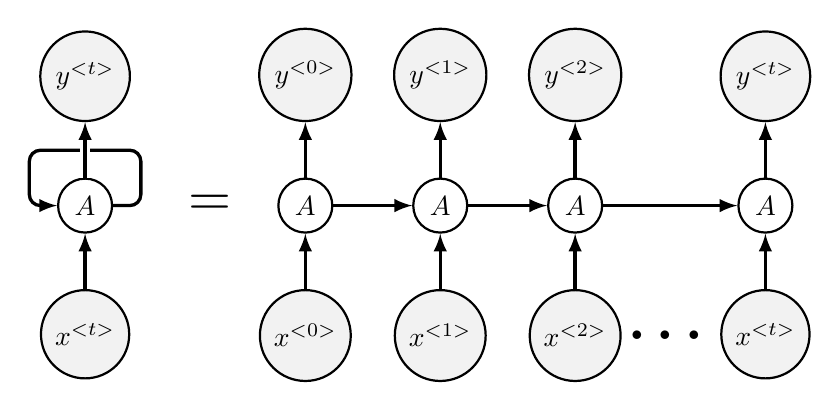
\begin{tikzpicture}[item/.style={circle,draw,thick,align=center},
        itemc/.style={item,on chain,join}]
      \begin{scope}
        [start chain=going right,nodes=itemc,every
          join/.style={-latex,very thick},local bounding box=chain]
        \path node (A0) {$A$} node (A1) {$A$} node (A2) {$A$} node[xshift=2em] (At) {$A$};
      \end{scope}
      \node[left=1em of chain,scale=2] (eq) {$=$};
      \node[left=2em of eq,item] (AL) {$A$};
      \path (AL.west) ++ (-1em,2em) coordinate (aux);
      \draw[very thick,-latex,rounded corners] (AL.east) -| ++ (1em,2em) -- (aux) |- (AL.west);
      \foreach \X in {0,1,2,t} {

        \draw[very thick,-latex] (A\X.north) -- ++ (0,2em) node[above,item,fill=gray!10]  (y\X) {$y^{<\X>}$};

        \draw[very thick,latex-] (A\X.south) -- ++ (0,-2em) node[below,item,fill=gray!10]  (x\X) {$x^{<\X>}$};
      }
      \draw[white,line width=0.8ex] (AL.north) -- ++ (0,1.9em);

      \draw[very thick,-latex] (AL.north) -- ++ (0,2em)
      node[above,item,fill=gray!10] {$y^{<t>}$};
      \draw[very thick,latex-] (AL.south) -- ++ (0,-2em)
      node[below,item,fill=gray!10] {$x^{<t>}$};
      \path (x2) -- (xt) node[midway,scale=2,font=\bfseries] {\dots};
    \end{tikzpicture}
    \item and the network is often initialized by random $A^{<0>}$ at the start of the network
    \item this type of model are called unidirection RNN, compared to bidirectional RNN where the paths moves both ways.
      \section{uni-directional RNN Forward propagation}
      \begin{description}
      \item $$a^{<t>} = g(W_{aa}a^{<t-1>} + W_{ax}X^{<t>} + b_a) $$
      \item $$\hat{y}^{<t>} = g(W_{ya}a^{<t>} + b_y) $$  where \textbf{g} function is usually \textbf{tanh}, or \textbf{relu}.
      \item  $a^{<t>}$ is usually represented in vectorized notation into  $$ a^{<t>} = g(W_{a}[A^{<t-1>}, X^{<t>}] + b_a) $$ where $W_a$ is $\begin{vmatrix}W_{aa} & {W_{ax}}\end{vmatrix}$, and $[a^{<t-1>}, X^{<t>}]=\begin{vmatrix} a^{<t-1>} \\ X^{<t>} \end{vmatrix}$
      \item $$ \hat{y}^{<t>} = softmax(W_{ya}a^{<t>} + b_y) $$
      \item $$L=\sum {L^{<t>}(\hat{y^{<t>}},y^{<t>})}$$

      \item notice that from the Bayesian chain-rule (see next chapter) that $P(y^{<t>}|y^{<1>}\dots{y^{<t-1>}})=\hat{y^{<t>}}$
        \section{uni-directional RNN backward propagation through time}
        \begin{description}
        \item (derive)
        \end{description}
        \section {Variations of RNN models}
        \begin{description}
        \item in the previous figure we discussed many-to-many uni-directional recurrent neural network architecture, a more general architecture is the bidirectional RNN where arrows goes both ways.
        \item another variation is many-to-one, and it look like this
          \subsection{many-to-one RNN}
          \begin{description}
        \item 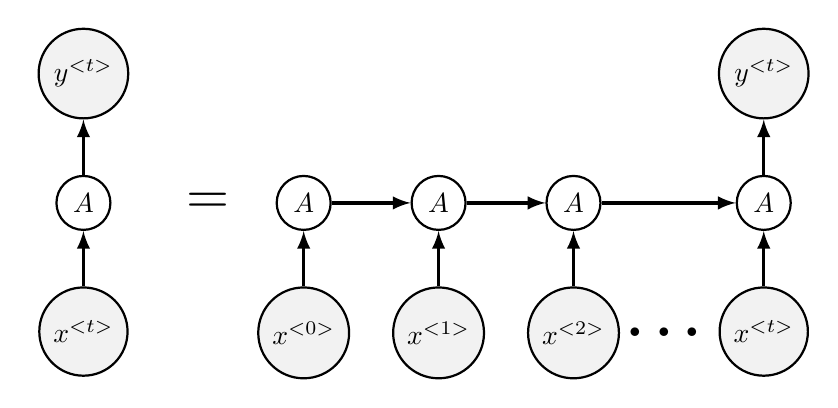
\begin{tikzpicture}[item/.style={circle,draw,thick,align=center},
        itemc/.style={item,on chain,join}]
      \begin{scope}
        [start chain=going right,nodes=itemc,every
          join/.style={-latex,very thick},local bounding box=chain]
        \path node (A0) {$A$} node (A1) {$A$} node (A2) {$A$} node[xshift=2em] (At) {$A$};
      \end{scope}
      \node[left=1em of chain,scale=2] (eq) {$=$};
      \node[left=2em of eq,item] (AL) {$A$};
      \path (AL.west) ++ (-1em,2em) coordinate (aux);
      %\draw[very thick,-latex,rounded corners] (AL.east) -| ++ (1em,2em) -- (aux) |- (AL.west);
      \draw[very thick,-latex] (At.north) -- ++ (0,2em) node[above,item,fill=gray!10]  (yt) {$y^{<t>}$};
      \foreach \X in {0,1,2,t} {
        \draw[very thick,latex-] (A\X.south) -- ++ (0,-2em) node[below,item,fill=gray!10]  (x\X) {$x^{<\X>}$};
      }
      \draw[white,line width=0.8ex] (AL.north) -- ++ (0,1.9em);
      \draw[very thick,-latex] (AL.north) -- ++ (0,2em)
      node[above,item,fill=gray!10] {$y^{<t>}$};
      \draw[very thick,latex-] (AL.south) -- ++ (0,-2em)
      node[below,item,fill=gray!10] {$x^{<t>}$};
      \path (x2) -- (xt) node[midway,scale=2,font=\bfseries] {\dots};
        \end{tikzpicture}
        \item notice that there is a single output the map the whole sequence to a single output, similar to the Neural network.
          \end{description}
          \subsection{One-to-Many RNN}
          \begin{description}
          \item and finally one-to-many, input to next time step is sampled from the previous output:
        \item 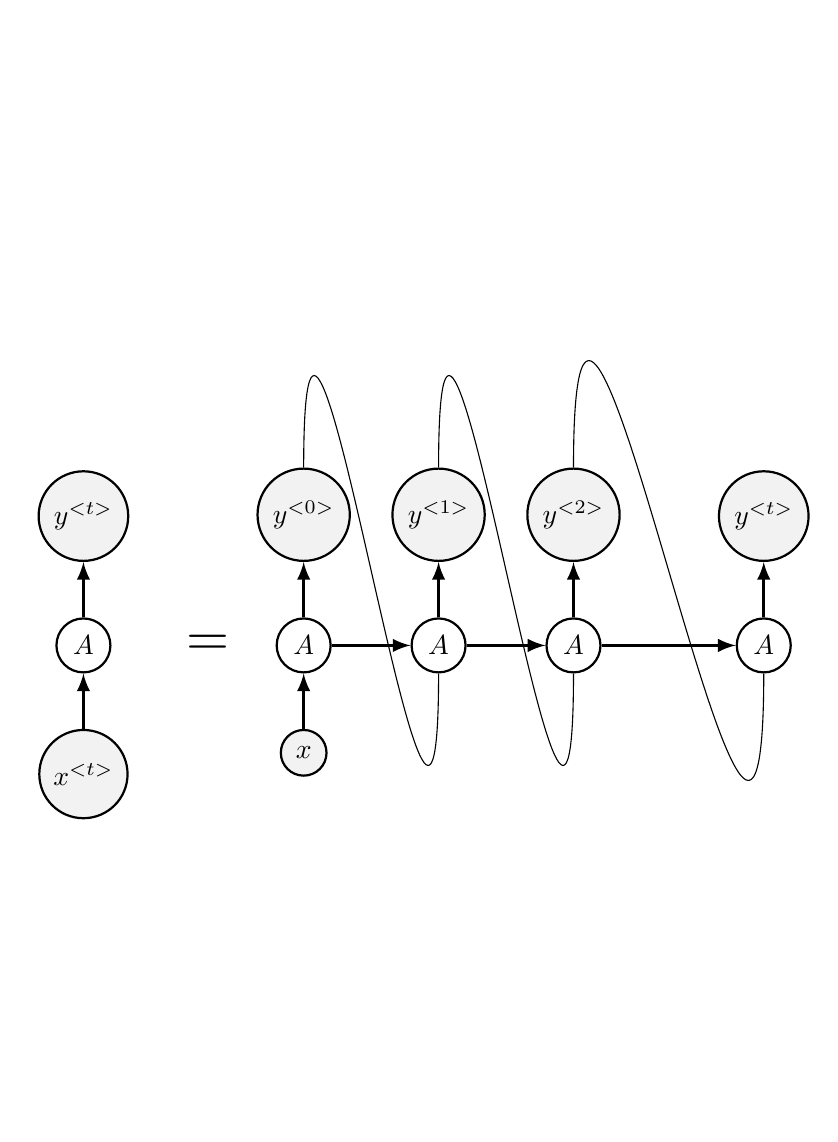
\begin{tikzpicture}[item/.style={circle,draw,thick,align=center},
        itemc/.style={item,on chain,join}]
      \begin{scope}
        [start chain=going right,nodes=itemc,every
          join/.style={-latex,very thick},local bounding box=chain]
        \path node (A0) {$A$} node (A1) {$A$} node (A2) {$A$} node[xshift=2em] (At) {$A$};
      \end{scope}
      \node[left=1em of chain,scale=2] (eq) {$=$};
      \node[left=2em of eq,item] (AL) {$A$};
      \path (AL.west) ++ (-1em,2em) coordinate (aux);
      \foreach \X in {0,1,2,t} {
        \draw[very thick,-latex] (A\X.north) -- ++ (0,2em) node[above,item,fill=gray!10]  (y\X) {$y^{<\X>}$};

      }

      \draw[very thick,latex-] (A0.south) -- ++ (0,-2em) node[below,item,fill=gray!10]  (x0) {$x$};
      \draw[white,line width=0.8ex] (AL.north) -- ++ (0,1.9em);

      \draw[very thick,-latex] (AL.north) -- ++ (0,2em)
      node[above,item,fill=gray!10] {$y^{<t>}$};
      \draw[very thick,latex-] (AL.south) -- ++ (0,-2em)
      node[below,item,fill=gray!10] {$x^{<t>}$};

      \draw (y0) to [out=90,in=270,looseness=4] (A1);
      \draw (y1) to [out=90,in=270,looseness=4] (A2);
      \draw (y2) to [out=90,in=270,looseness=4] (At);

        \end{tikzpicture}
        \item for example in a music generation model, the input X could be the genre, or the initial note, or could pi ${\phi}$.
          \end{description}
          \end{description}
        \subsection{Many-to-Many of different input/output length}
        \begin{description}

        \item \begin{tikzpicture}[item/.style={circle,draw,thick,align=center},
        itemc/.style={item,on chain,join}]
      \begin{scope}
        [start chain=going right,nodes=itemc,every
          join/.style={-latex,very thick},local bounding box=chain]
        \path node (A0) {$A$} node (A1) {$A$} node (A2) {$A$} node[xshift=2em] (At) {$A$};
      \end{scope}
      \node[left=1em of chain,scale=2] (eq) {$=$};
      \node[left=2em of eq,item] (AL) {$A$};
      \path (AL.west) ++ (-1em,2em) coordinate (aux);

      \draw[very thick,latex-] (A0.south) -- ++ (0,-2em) node[below,item,fill=gray!10]  (x0) {$x^{<0>}$};

      \draw[very thick,latex-] (A1.south) -- ++ (0,-2em) node[below,item,fill=gray!10]  (x1) {$x^{<n>}$};
      \path (x0) -- (x1) node[midway,scale=0.5,font=\bfseries] {\dots};
      \draw[very thick,-latex] (A2.north) -- ++ (0,2em) node[above,item,fill=gray!10]  (yn) {$y^{<n>}$};
      \draw[very thick,-latex] (At.north) -- ++ (0,2em) node[above,item,fill=gray!10]  (yt) {$y^{<t>}$};
      \path (x2) -- (xt) node[midway,scale=2,font=\bfseries] {\dots};
      \draw[white,line width=0.8ex] (AL.north) -- ++ (0,1.9em);
      \draw[very thick,-latex] (AL.north) -- ++ (0,2em)
      node[above,item,fill=gray!10] {$y^{<t>}$};
      \draw[very thick,latex-] (AL.south) -- ++ (0,-2em)
      node[below,item,fill=gray!10] {$x^{<t>}$};
        \end{tikzpicture}
          \item (TODO fix the spacing)
        \item in the case of machine translation, the model in composed of encoder consisting of the first input $X^{<0>}$ to $X^{<n>}$, and output decoder consisting of the last output $y^{<n+1>}$ to $y^{<t>}$.
        \end{description}
      \item (TODO add attention based architecture)

      \end{description}

    \end{description}

    \section{Language Model and sequence generation}
    \begin{description}
    \item In NLP sequence generation the many-to-many model of the same length is utilized, where each input (one-hot vector) representation of the word $X^{<t>}$ maps to $Y^{<t>}$: the probability of an input word given the prior words, can be the output of a \textbf{softmax} activation into the whole indices of the vocabulary.
    \item after training the model on a large training example, the output sequence can be utilized to predict the most likely word after a given input sequence, for example for a new input sequence $y^{<1>}, y^{<2>}, y^{<3>}$, what is $P(y^{<1>}, y^{<2>}, y^{<3>})$, using the chain-rule (see the appendix on probabilities) this term expands to $P(y^{<1>})P(y^{<2>}|y^{1})P(y^{<3>}|y^{<2>},y^{<1>})=\hat{y^{<1>}}\hat{y^{<2>}}\hat{y^{<3>}}$
    \end{description}
    \section{Sampling novel sequences}
    \begin{description}
    \item it's possible to generate a novel sequence from the trained weights from a corpus, for example if the initial node $a^{<0>}=X^{<0>}=0$, and the input $X^{<1>} \to X^{<T_x>}$ are taken from the previous output $y^{<0>} \to X^{<T_y-1>}$, for example $X^{<t>}=y^{<t-1>}$, then it output a sequence with writing style, and vocabulary similar to that of the corpus.
    \item so if the the corpus vocabulary contain <EOS> or end of sentence token, sequence generator can stop after <EOS>, otherwise, it can set to generate a specific length of words (we will discuss pre-processing in NLP chapter).
    \item in previous case the input is a vocabulary of words, it could be modeled on sequence of characters instead in similar way, in this case the vocabulary is the set of characters, and numbers, white space, and possibly punctuation.
    \end{description}
    \section{Vanishing/Exploding gradients}
    \begin{description}
    \item similar to the Neural network, RNN also can have Vanishing, and exploding gradients, it turns out that the latter is less common, in this case it leads to overflow of output, and usually solved by gradient clipping, or comparing the output against some threshold, then re-scale the gradient vector as to normalize it, but the former case of vanishing gradients is the most common, in a very long model.
      \subsection{Gated Recurrent Unit (GRU)}
      \begin{description}
      \item starting with an example from NLP, in English language, verbs are conjugated w.r.t the subject in the sentence, in a very long text, keeping track of the subject is essential, but in the RNN which flows from the left to right can be substantially long, such  forward, and backward propagation influences the advanced nodes is very negligible thus leading to vanishing gradients problems, to solve this, keeping a record of the such pivotal words is essential, for this GRU was invented.

      \item (TODO draw GRU graph)
        \subsection{GRU simplified}
        \begin{description}
        \item define memory cell C, $C^{<t-i>} = a^{<t-i>}$.
        \item an estimate of the $C^{<t>}$ is notated with  $\tilde{C^{<t>}}$.
        \item the the estimated C is gated with $\Gamma_u$ (update gate, sometimes denoted by $\Gamma_i$), multiplied together to generate the output $C^{<t>}$.
        \item $$\tilde{C^{<t>}}=tanh(W_c[c^{<t-1>},X^{<t>}]+b_c) $$
        \item $$ \Gamma_u = \sigma(W_u[c^{<t-1>},X^{<t>}]+b_u) $$
        \item $$ C^{<t>}=\Gamma_u * \tilde{C^{<t>}} + (1-\Gamma_U)*C^{<t-1>}$$ (note that * denotes element-wise multiplication).
        \end{description}
      \end{description}
    \item for a full GRU implementation relevance gate $\Gamma_r$ is used to estimate the relevance of $C^{<t-1>}$ to calculate $\tilde{C^{<t>}}$
    \item \item $$ \Gamma_r = \sigma(W_r[c^{<t-1>},X^{<t>}]+b_u) $$
    \item $$\tilde{C^{<t>}}=tanh(W_c[\Gamma_r*c^{<t-1>},X^{<t>}]+b_c) $$
    \end{description}
    \subsection{Long Short Term Memory (LSTM)}
    \begin{description}
    \item 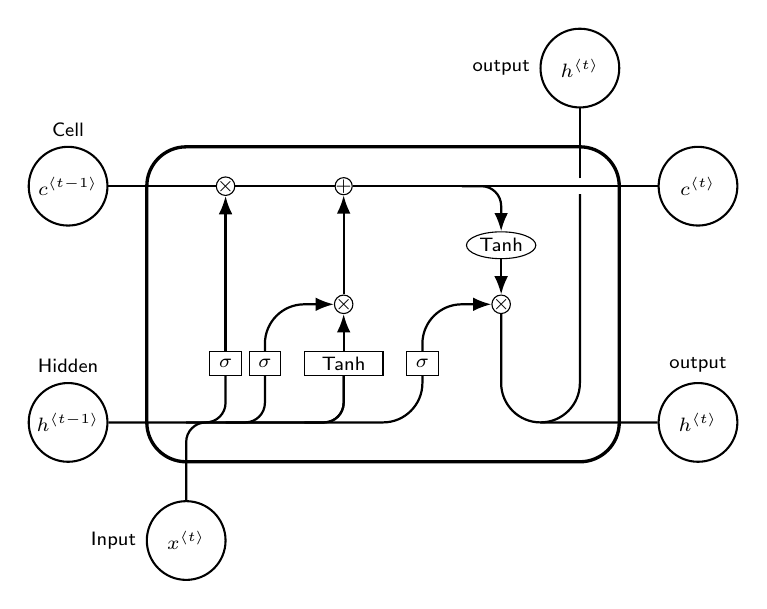
\begin{tikzpicture}[
        % GLOBAL CFG
        font=\sf \scriptsize,
        >=LaTeX,
        % Styles
        cell/.style={% For the main box
          rectangle,
          rounded corners=5mm,
          draw,
          very thick,
        },
        operator/.style={%For operators like +  and  x
          circle,
          draw,
          inner sep=-0.5pt,
          minimum height =.2cm,
        },
        function/.style={%For functions
          ellipse,
          draw,
          inner sep=1pt
        },
        ct/.style={% For external inputs and outputs
          circle,
          draw,
          line width = .75pt,
          minimum width=1cm,
          inner sep=1pt,
        },
        gt/.style={% For internal inputs
          rectangle,
          draw,
          minimum width=4mm,
          minimum height=3mm,
          inner sep=1pt
        },
        mylabel/.style={% something new that I have learned
          font=\scriptsize\sffamily
        },
        ArrowC1/.style={% Arrows with rounded corners
          rounded corners=.25cm,
          thick,
        },
        ArrowC2/.style={% Arrows with big rounded corners
          rounded corners=.5cm,
          thick,
        },
      ]

      %Start drawing the thing...
      % Draw the cell:
      \node [cell, minimum height =4cm, minimum width=6cm] at (0,0){} ;

      % Draw inputs named ibox#
      \node [gt] (ibox1) at (-2,-0.75) {$\sigma$};
      \node [gt] (ibox2) at (-1.5,-0.75) {$\sigma$};
      \node [gt, minimum width=1cm] (ibox3) at (-0.5,-0.75) {Tanh};
      \node [gt] (ibox4) at (0.5,-0.75) {$\sigma$};

   % Draw opérators   named mux# , add# and func#
    \node [operator] (mux1) at (-2,1.5) {$\times$};
    \node [operator] (add1) at (-0.5,1.5) {+};
    \node [operator] (mux2) at (-0.5,0) {$\times$};
    \node [operator] (mux3) at (1.5,0) {$\times$};
    \node [function] (func1) at (1.5,0.75) {Tanh};

    % Draw External inputs? named as basis c,h,x
    \node[ct, label={[mylabel]Cell}] (c) at (-4,1.5) {\empt{c}{t-1}};
    \node[ct, label={[mylabel]Hidden}] (h) at (-4,-1.5) {\empt{h}{t-1}};
    \node[ct, label={[mylabel]left:Input}] (x) at (-2.5,-3) {\empt{x}{t}};

    % Draw External outputs? named as basis c2,h2,x2
    \node[ct, label={[mylabel]}] (c2) at (4,1.5) {\empt{c}{t}};
    \node[ct, label={[mylabel]output}] (h2) at (4,-1.5) {\empt{h}{t}};
    \node[ct, label={[mylabel]left:output}] (x2) at (2.5,3) {\empt{h}{t}};

% Start connecting all.
    %Intersections and displacements are used.
    % Drawing arrows
    \draw [ArrowC1] (c) -- (mux1) -- (add1) -- (c2);

    % Inputs
    \draw [ArrowC2] (h) -| (ibox4);
    \draw [ArrowC1] (h -| ibox1)++(-0.5,0) -| (ibox1);
    \draw [ArrowC1] (h -| ibox2)++(-0.5,0) -| (ibox2);
    \draw [ArrowC1] (h -| ibox3)++(-0.5,0) -| (ibox3);
    \draw [ArrowC1] (x) -- (x |- h)-| (ibox3);

    % Internal
    \draw [->, ArrowC2] (ibox1) -- (mux1);
    \draw [->, ArrowC2] (ibox2) |- (mux2);
    \draw [->, ArrowC2] (ibox3) -- (mux2);
    \draw [->, ArrowC2] (ibox4) |- (mux3);
    \draw [->, ArrowC2] (mux2) -- (add1);
    \draw [->, ArrowC1] (add1 -| func1)++(-0.5,0) -| (func1);
    \draw [->, ArrowC2] (func1) -- (mux3);

    %Outputs
    \draw [-, ArrowC2] (mux3) |- (h2);
    \draw (c2 -| x2) ++(0,-0.1) coordinate (i1);
    \draw [-, ArrowC2] (h2 -| x2)++(-0.5,0) -| (i1);
    \draw [-, ArrowC2] (i1)++(0,0.2) -- (x2);

\end{tikzpicture}
    \item $$\tilde{C^{<t>}}=tanh(W_c[c^{<t-1>},X^{<t>}]+b_c) $$
    \item $$ \Gamma_u = \sigma(W_u[a^{<t-1>},X^{<t>}]+b_u) $$
    \item $$ \Gamma_f = \sigma(W_f[a^{<t-1>},X^{<t>}]+b_f) $$ is the forget gate used instead of $(1-\Gamma_u)$.
    \item $$ \Gamma_o = \sigma(W_o[a^{<t-1>},X^{<t>}]+b_o) $$ is the output gate
    \item $$ C^{<t>}=\Gamma_u * \tilde{C^{<t>}} + \Gamma_f*C^{<t-1>}$$
    \item $$ a^{<t>} = \Gamma_o * tanh(C^{<t>})$$.
    \item one notice here is that in $\Gamma_o$ instead of $X^{<t>}$ you could use $C^{<t-1>}$ instead, and known as \textbf{peephole connection}
      \subsection{Back-propagation}
      \begin{description}
      \item (TODO add derivation)
      \end{description}
    \end{description}
    \subsection{Bidirectional RNN}
    \begin{description}
      \item bidirectional RNN runs forward propagation both forward, and backward, utilizing two activation unites $a_f^{<t>}$, and $a_b^{<t>}$, instead of just $a^{<t>}$, where the propagation flows from $a_f^{<i>} \rightarrow a_f^{<i+1>}$, at the same time, from $a_b^{<i+1>} \leftarrow a_b^{<i>}$, to estimate $$\hat{y^{<t>}} = g(W_y\begin{vmatrix}a_f^{<t>}\\a_b^{<t>}\end{vmatrix} + b_y)$$.
      \item 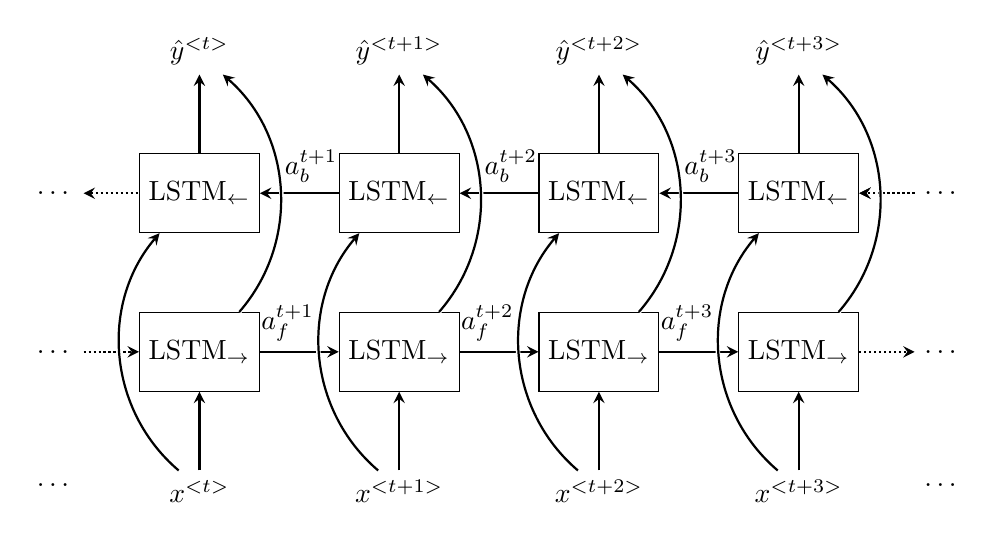
\begin{tikzpicture}
	\node[rectangle] (Y0) at (0, 0) {$\dots$};
	\node[rectangle, draw, right=2em of Y0, minimum height=1cm, minimum width=1cm] (RNN) {LSTM$_\rightarrow$};
	\node[rectangle, right=of RNN, draw, minimum height=1cm, minimum width=1cm] (RNN2) {LSTM$_\rightarrow$};
	\node[rectangle, right=of RNN2, draw, minimum height=1cm, minimum width=1cm] (RNN3) {LSTM$_\rightarrow$};

	\node[rectangle, right= of RNN3, draw, minimum height=1cm, minimum width=1cm] (RNN4) {LSTM$_\rightarrow$};
	\node[rectangle, right=2em of RNN4] (RNN5) {$\dots$};


	\node[rectangle, above=of RNN4, draw, minimum height=1cm, minimum width=1cm] (R25) {LSTM$_\leftarrow$};
	\node[rectangle, left=of R25, minimum height=1cm, minimum width=1cm, draw] (R24) {LSTM$_\leftarrow$};
	\node[rectangle, left=of R24, draw, minimum height=1cm, minimum width=1cm] (R23) {LSTM$_\leftarrow$};
	\node[rectangle, left=of R23, draw, minimum height=1cm, minimum width=1cm] (R22) {LSTM$_\leftarrow$};
	\node[rectangle, left=2em of R22] (R21) {$\dots$};
	\node[right=2em of R25] (Y20) {$\dots$};

	\node[below=of RNN] (X1) {$x^{<t>}$};
	\node[below=of RNN2] (X2) {$x^{<t+1>}$};
	\node[below=of RNN3] (X3) {$x^{<t+2>}$};
	\node[below=of RNN4] (X4) {$x^{<t+3>}$};
	\node[above=of R25] (Y5) {$\hat{y}^{<t+3>}$};
	\node[above=of R24] (Y4) {$\hat{y}^{<t+2>}$};
	\node[above=of R23] (Y3) {$\hat{y}^{<t+1>}$};
	\node[above=of R22] (Y2) {$\hat{y}^{<t>}$};

	\draw[-stealth, thick] (X1) -- (RNN);
	\draw[-stealth, thick] (X2) -- (RNN2);
	\draw[-stealth, thick] (X3) -- (RNN3);
	\draw[-stealth, thick] (X4) -- (RNN4);
	\draw[-stealth, thick, densely dotted] (Y0) -- (RNN);
	\draw[-stealth, thick] (RNN) -- node[above, pos=0.35] {$a_f^{t+1}$} (RNN2);
	\draw[-stealth, thick] (RNN2) -- node[above, pos=0.35] {$a_f^{t+2}$} (RNN3);
	\draw[-stealth, thick] (RNN3) -- node[above, pos=0.35] {$a_f^{t+3}$} (RNN4);
	\draw[-stealth, densely dotted, thick] (RNN4) -- (RNN5);
	\node[below=4em of Y0] (d) {\dots};
	\node[below=4em of RNN5] (d) {\dots};

	\path[-stealth, ultra thick, white] (X1) edge[bend left=45] (R22);
	\path[-stealth, thick] (X1) edge[bend left=45] (R22);
	\path[-stealth, ultra thick, white] (X2) edge[bend left=45] (R23);
	\path[-stealth, thick] (X2) edge[bend left=45] (R23);
	\path[-stealth, ultra thick, white] (X3) edge[bend left=45] (R24);
	\path[-stealth, thick] (X3) edge[bend left=45] (R24);
	\path[-stealth, ultra thick, white] (X4) edge[bend left=45] (R25);
	\path[-stealth, thick] (X4) edge[bend left=45] (R25);
	\draw[-stealth, densely dotted, thick] (Y20) -- (R25);

	\draw[-stealth, thick] (R22) -- (Y2);
	\draw[-stealth, thick] (R23) -- (Y3);
	\draw[-stealth, thick] (R24) -- (Y4);
	\draw[-stealth, thick] (R25) -- (Y5);

	\draw[stealth-, densely dotted, thick] (R21) -- (R22);
	\draw[stealth-, thick] (R22) -- node[above, pos=0.65] {$a_b^{t+1}$} (R23);
	\draw[stealth-, thick] (R23) -- node[above, pos=0.65] {$a_b^{t+2}$} (R24);
	\draw[stealth-, thick] (R24) -- node[above, pos=0.65] {$a_b^{t+3}$} (R25);
	\draw[-stealth, densely dotted, thick] (Y20) -- (R25);

	\path[-stealth, ultra thick, white] (RNN) edge[bend right=45] (Y2);
	\path[-stealth, thick] (RNN) edge[bend right=45] (Y2);
	\path[-stealth, ultra thick, white] (RNN2) edge[bend right=45] (Y3);
	\path[-stealth, thick] (RNN2) edge[bend right=45] (Y3);
	\path[-stealth, ultra thick, white] (RNN3) edge[bend right=45] (Y4);
	\path[-stealth, thick] (RNN3) edge[bend right=45] (Y4);
	\path[-stealth, ultra thick, white] (RNN4) edge[bend right=45] (Y5);
	\path[-stealth, thick] (RNN4) edge[bend right=45] (Y5);
      \end{tikzpicture}

    \item this model require first processing all the sequence input, before generating any output, with advantage of both backward, and forward contextual semantics awareness, and disadvantage that output is generated after processing all the input X.
    \end{description}
    \section{Deep RNNs}
    \begin{description}
    \item (TODO insert the graph)
    \item (TODO add forward/backward propagation)
    \end{description}
  \end{description}
  \section{Word Representation}
  \begin{description}
  \item previously we discussed one-hot vector representation of a word in NLP models( we will elaborate more on that in following chapters), as a representation of a word in vector of size V, which is the length of the vocabulary, each word is denoted by $O_{word index}$, but this sparse representation have drawbacks, that the dot product(degree of alignment) isn't captured, so any two words, no matter how similar will have zero dot product,  for example the pair Man/Woman, King/Queen, Apple/Orange aren't distinguished from each others, instead a high dimensional featured representation is used coined \textbf{Word Embedding}.
    \subsection{Word Embedding}
    \begin{description}
    \item word embedding for dictionary V is a matrix where each word is represented by a column vector matched against features at each row. in this case, we can use rules of Linear Algebra applied on word embedding representation, as for example to calculate the distance between two different words, so in the pair Queen/King, or Woman/man we expect the distance between the words in each pair to be the same with negligible difference, and this distance is called \textbf{Cosine Similarity}  (we will elaborate on that in following chapters).
      \subsection{Named Entity recognition}
      \begin{description}
      \item in the following two sentences \begin{enumerate}
      \item Sally Johnson is an orange farmer.
      \item Robert Lin is an apple farmer.
      \end{enumerate}
      \item only with word Embedding a trained BRNN model on a large text corpus, where it encounter the first sentence, can deduce from the second example the ``Robert Lin'' is a name of person.
      \item to use such model, it first trained on large data-set, then with transfer learning, new tasks are added with moderate size data-set for example 100k words, as analogous to convolution NN in computer vision, where a trained model with large data-set can be utilized with image encoding to generalize to new task.

      \end{description}
      \item for a Vocabulary of V words, the \textbf{Matrix Embedding} $E$ of N-dimensional features, is consistent of V word embedding, for example for word $w^i$, if it's embedding it's $e_{w^i}$, then $EO_{w^i}=e_{w^i}$ of size N.
        \subsection{Learning word embedding}
        \begin{description}
        \item How word embedding is generated for a new word? given Matrix Embedding?
          %TODO add a graph representation
        \item In a sequence of words $w_1,w_2,\dots,w_{n_1}$, prediction of the \textbf{nth} word $w_n$ can be the output of a Neural Network, feed by window \textbf{W} of preceding word embedding, given a Matrix Embedding E of N features, and sentence, with corresponding one-hot vector representation of \textbf{V} words vocabulary  , each vector work embedding $e_{w^i}$ is calculated, and feed as input to the neural network. the final neural network would be of input size $W\times{N}$, feed to neural network of L layers (usually 1 layer), with final SOFTMAX output of length V, and produces the predicted one-hot vector representation of the \textbf{nth} word $w_n$.
          \subsection{Word2Vec}
            \subsection{Skip gram}
            \begin{description}
            \item skip-gram word embedding generation fixated a target word $w_t$, or for simplicity, rather than feeding the preceding sequence in window W, it randomly samples a context word $w_c$, or c for simplicity, from a window of length \textbf{W}, with equal length input/output layers, with middle SOFTMAX activation layer.

              \subsection{hierarchical SOFTMAX}
              \begin{description}
                %TODO elaborate more! check the paper.
              \item for a small vocabulary V of even 10k words, generating a word embedding for each words $P(w_t|w_c)$ can be quite expensive summing over the entire vocabulary for each target word: $$ p(w_t|w_c) = \frac{e^{\theta_t^Te_c}}{\sum_{j=1}^Ve^{\theta_j^Te_c}}$$ notice here the bias term is ignored, where $\theta_k$ is the weight parameter associated with word $w_k$ for i $\in$ [1\text{-}V]. so instead the hierarchical SOFTMAX sorts the context words in tree, and uses a binary-search-like algorithms to narrow down the search to closest word region.
                %thus summing over smaller range
                \item
              \item secondly in the random sampling, the heuristic is not to choice uniformly, ending up repeating the calculation for the most frequent words for example the STOP words ``the'', or ``of'' as context words.
                \end{description}
            \end{description}
            \subsection{Negative Sampling}
            \begin{description}
            \item another variant, yet faster than SOFTMAX embedding generation network is Negative Sampling, it solves the expensive activation, so instead of summing over the whole Vocabulary, the window of K words from a data-set of input X context/target words map, and output binary vector Y, $$ \begin{cases} 1 \leftarrow \text{context and target matches}\\ 0 \leftarrow \text{otherwise} \end{cases} $$
            \item the sampling of the k words is chosen from the distribution: $$ P(w_i) = \frac{f(w_i)^{\frac{3}{4}}}{\sum_{j=1}^{V}f(w_j)^{\frac{3}{4}}} $$ for f being the frequency function, (this proven to be efficient).
            \item k is changed depending on the size of the data-set for a small data-set it usually 5-20, for large-dataset, it's less then 5, for example the input vector for the target word $w_t$ from randomly chosen context words with X-Y being for example: $$\begin{vmatrix}w_c^1\\w_c^2\\ \vdots\\w_c^k\end{vmatrix}  \rightarrow \begin{vmatrix}1\\0\\ \vdots\\0\end{vmatrix}$$,
              \item for a given data-set, it's possible to randomly choose words from the dictionary, and assign it as negative (with value zero), and added it to the X-Y mapping,
              \item then similar to the skip-gram algorithm, the embedding of each word vector is feed to the neural network, but instead of softmax activation, logistic activation used instead: $$ P(y=1|c,t) = \sigma(\theta_t^Te_c) $$
            \end{description}
            \subsection{GloVe (global vector for word representation)}
            \begin{description}
            \item even simpler word representation is the GloVe algorithm, a descent of the neural word embedding, and skip-gram.
            \item for a specific context function, input X, is the frequency of the one target word appearing in the context of another, such that $X_{ij}$ is the frequency of the $w_j$ appearing in the context of $w_i$.
            \item Glove cost function is thus defined as follows $$ J(\theta, e) = \sum_{i=1}^V\sum_{j=1}^Vf(X_{ij})(\theta_i^Te_j + b_i + b_j - log(X_{ij}))^2 $$
            \item in gradient descent both the weight $\theta$, and the embedding e are updated, moreover after each word, the embedding is normalized as follows $e_w=\frac{e_w+\theta_w}{2}$
            \item it's worth noting that for invertible matrix A, a transformation over the vector space of the embedding $(A\theta_i)^T(A^{-T}e_j)=\theta_i^Te_j$, meaning different transformation over the embedding vector can lead to the same evaluation of the cost, and therefore with different interpretations on the single vector space, that doesn't guarantee that specific embedding will be human-interpretable.
            \end{description}
        \end{description}
    \end{description}
    \section{Example: Sentiment Classification}
    \begin{description}
    \item for a sequence of N words review, for example a review of a product, ignoring the sequence order, the problem can be modeled in a simple SOFTMAX activation layer of the average, or sum of the embedding of the sequence words $ z = \sum_{i=1}^Ne_i $, while Y is a 5 star classification vector of length 5, $Z=W^Taverage(X) + b$, $\hat{y} = softmax(Z)$, $L=Y.log(\hat{Y)}$ the problem with this model, it fails to accurately classify long sentences, sentences that aren't straight-forward, to maintain the sequence, many-to-one RNN is used instead, and feed with the word embedding as the input,  with output softmax layer.
    \end{description}
    \section{Sequence To Sequence Model}
    \begin{description}
      % TODO does beam search reduces the computational cost?!
      % if the beam length=1, then it's a greedy search!
      % it seams the it increase the cost, but
      % a gready search is V^{sentence length}, while
      % beam search is 3*V*{sentence length}, or i'm wrong?!
      % if i'm right then 1*V*{sentence length} is the computational cost, and that is a contradiction, so something is wring in those assumptions 1,2.
    \item sequence to sequence model is a generative model, generating an output sequence $y^{<1>}\text{-}y^{<T_y>}$, or $$P(y^{<1>},\dots,y^{<Ty>}|x^{<1>},\dots,x^{<Tx>})$$ from input sequence $x^{<1>}\text{-}x^{<T_x>}$, an interesting example is image captioning, taking Alexnet network SOFTMAX output, can fit as a an input sequence, to be trained on captioning data-set. for example $T_x$ can be softmax of length 4096, and $T_x$ is the captioning length can be set to 10 words.
    \item a single input sequence \textbf{X} can map to different possible output sequence \textbf{Y}, sequence to sequence model aim for the maximum probability $$\underset{y^{<1>},\dots,y^{<T_Y>}}{\operatorname{argmax}}\prod_{t=1}^{T_y}P(y^{<t>}|X,y^{<1>},\dots,y^{<t-1>})$$.
    \item to explain the complexity analysis, let's pick an example, for example in NLP machine translation, the greedy search approach for this argmax has complexity of $O(V^{T_y})$, where V is the vocabulary size, for example in a output as small as 10 sequence words, from a moderate vocabulary of length 100k, then the sample space is $100000^{10}$ ! which is infeasible for a moderate application, instead a non-optimal heuristic search algorithm is usually employed for example  \textbf{beam search}.
      \subsection{Beam search}
      \begin{description}
      \item noticing in the previous example the in almost all cases, in machine translation example from a vocabulary of size V, only a small fraction of words can have reasonable probability, so it's possible to set a Window/Width \textbf{W} for example of $W=5$ words to search instead of the whole vocabulary at the initial step, so to instantiate the network N times, so at first sequence $Y^{<1>}$ there are only W possibilities are fit  $P(y^{<1>}|X)$, similarly at second step $Y^{<2>}$ there are equivalently maximum W words $P(y^{<1>},y^{<2>}|X)$, at the second step another instantiation of the network , leading to step 3, for sequence  $Y^{<3>}$, $P(y^{<1>},y^{<2>},y^{<3>}|X)$, and so on, this shrink down the complexity to $O(W\times{V}\times{T_y})$.
        \subsection{normalization}
        \begin{description}
        \item in a long sequence model, the argmax output for a small values of X,Y can quickly diminishes to zero, to prevent this, the mean the log of the likelihood is implemented instead: $$
          \underset{y^{<1>},\dots,y^{<T_Y>}}{\operatorname{argmax}}\frac{1}{T_y^{\alpha}}\sum_{t=1}^{T_y}logP(y^{<t>}|X,y^{<1>},\dots,y^{<t-1>})$$ (note that $\alpha$ is tuning parameter).
        \end{description}
        \item beam search is non-optimal compared to DFS, or BFS algorithms, but with advantage of being faster, and the reason for that, is it never search the whole sequence space.
        \item how to choose the beam Width? beam width is a trade-off between speed, and accuracy, in practice it's usually in the range 5\textbf{-}10.
          \subsection{Error Analysis}
          \begin{description}
          \item in many-to-many RNN network employing Beam search, it could be that the window/width of beams search at fault, or the RNN at fault, to decide it wise to keep a boolean flag for the following to look at during development, given an input sequence X, and ground truth table output Y, the beam search is at fault, if for the output $\hat{Y}$, $P(Y|X)>P(\hat{Y}|X)$, otherwise, then the RNN is at fault.
          \end{description}
          \subsection{Bleu Score}
          \begin{description}
          \item the previous example still proceeds to explain Bleu Score metric which is essential for such example where the output sequence can take different valid output, for example for input sentence, from English language, the Spanish translation, can varies, to evaluate the machine translation MT, against human translation references, through combined bleu score: $$ Bp\textbf{ exp}(\frac{1}{4}\sum_{n=1}^4P_n) $$ where \textbf{Bp} is coined brevity penalty, and defined as $$\begin{cases} 1 | \text{  if length of MT $>$ reference length} \\ exp(\frac{1-\text{reference length}}{\text{MT length}}) | \text{  otherwise}\end{cases}$$
          \item bleu score $p_n$ for set for references output, and MT output, defined using two function, count for counting the n-grams in the MT combined, and references, and $count_{clip}$ for counting the number of \text{n-grams} in any of the references, and thus defined as: $$ p_n = \frac{\sum_{\text{n-gram} \in \hat{y}} Count_{clip}(\text{n-gram})}{\sum_{\text{n-gram} \in \hat{y}} Count(\text{n-gram})} $$
          \end{description}
      \end{description}
    \end{description}
  \end{description}
  \section{Attention Model}
  \begin{description}
    \item first let the bi-directional RNN output for time step t be $a^{<t>}=(a_f^{<t>},a_b^{<t>})$
    \item attention model takes the output sequence of a bi-directional RNN $a^{<1>},a^{<2>},\dots,a^{<T_x>}$ as the input sequence of a second layer LSTM-RNN (called hidden state S) , where each output is associated with attention/weights given to K input sequences $a^{<t>},a^{<t+1>},\dots,a^{<t+k>}$, and output sequences, $\begin{bmatrix}\alpha^{<t,t`>} \\ \alpha^{<t,t`+1>}\\ \vdots \\ \alpha^{<t,t`+k>}\end{bmatrix}$ the first layer is initialized with $a^{<0>}$, and second hidden state layer is initialized with $s^{<0>}$ (note the second index is for input sequence, and first index is the index of the second LSTM layer index).
      \subsection{Attention}
      \begin{description}
    \item the attention commit to  the following constraints, $\sum_t\alpha^{<t`,t>}=1$ for all t` time steps. and the input to the second RNN layer $c^{<t>}=\sum_t\alpha^{<t,t`>}a^{<t>}$ for all $t`$.
    \item since the attention is dependent on the current state at time $t`$ for the output of first LSTM layer, and the previous state of the hidden layer, and since this parameter isn't known, a softmax activation is used to train, and estimate this parameter $e^{<t,t`>}$, in order to calculate $$\alpha^{<t,t`>} = \frac{exp(e^{<t,t`>})}{\sum_{t`=1}^{T_x}exp(e^{<t,t`>})} $$ and the parameter $e^{<t,t`>}(a^{<t`>}, s^{<t-1>})$ is estimated for each time step.
      \end{description}


    \end{description}


  \chapter{Probabilistic Graphical Models (PGM)}
  \section{Introduction}
  \begin{description}
  \item first, what Models are? models are declarative representation of the world, \textbf{probabilistic models:} are representation of the uncertainty of the model. PGM is graphical representation of a phenomena, that can be used with other input data with other algorithms to take decisions, in classification, segmentation, or  recognition. and the reasons for uncertainty : \begin{enumerate}
  \item partial knowledge of state of the world
  \item noisy observations
  \item phenomena not covered by the model
    \item inherent stochasticity: that the world is inherently stochastic, and therefor the model.
  \end{enumerate}
  \item therefore the model is probabilistic and feed with random input variables mimicking uncertainty with their joint distribution.
  \item examples on graph are Bayesian network, represented with directed graph, and Markov networks (un-directed graph, usually weighted).
    \subsection{preliminaries}
    \begin{description}
    \item given random variables (for example I,D,G, being the data sampled from a class I(intelligence), D(difficulity), G(grade) the joint distribution P(I,D,G),and represented as a vector of joint distribution.
    \item \textbf{reduced random variable}: is the joint distribution under certain conditions for subset of the random variables for example $p(I,D,G^1)$ of the binary random variable G(taking the values 0,1), $G^1$ is the random variable $G=1$. and $p(I,D,G^1)$ is the reduced distribution to $G^1$ values.
    \item \textbf{re-normalized RV}: is the process of normalizing the distribution after reduction.
    \item \textbf{marginalization of RV}: is the distribution of one RV summed over the distribution of another for example $P(D)=\sum_{i=1}^nP(D|I)$.
      \subsection{factors}
      \begin{description}
      \item consider the vector variables A,B,C with arbitrary values called scope, factor are the building block, or the input for our model for probabilistic representation in high-dimensional spaces.
      \item \textbf{factor} is a map from set of random variable \textbf{scope}(parameters) to real value $\phi(X^0,X^1,...,X^n) \rightarrow \mathbb{R}$ for example the joint distribution $P(I,D,g^1)$ is a factor, and the scope in the case is I,D since $g^1$ is set to $g^1$ binary random variable constant value, factors aren't necessarily of probability scope, but could be for any values.
      \item \textbf{factor product}:  $\phi_1{(A,B)} \phi_2{(B,C)}=\phi_3{(A,B,C)}$ multiplication done on the real scalar values.
      \item \textbf{factor marginalization}: from distribution $\phi{(A,B,C)}$, to marginalize over B, $\phi{(A,C)}=\sum_{i=1}^{n={\#B}}\phi(A,C)$ ($\#B$ means size of variable B).
      \item \textbf{reduced factor}: reduced factor over $C^1$ is $\phi{(A,B,C^1)}=\phi{(A,B,C)} \leftarrow {C=1}$.
      \end{description}
    \item \textbf{Conditional Probability Distribution (CPD}): is the conditional probability with a joint probability distribution, for example $P(G|I,D)$.

    \end{description}
    \section{Bayesian Network Fundamentals}
    \begin{description}
    \item for student grading with vector random variables, G(grades),D(course difficulity),I(intelligence),S(sat score),L(reference recommendation letter).
      \subsection{constructing dependencies}
      \begin{description}
      \item  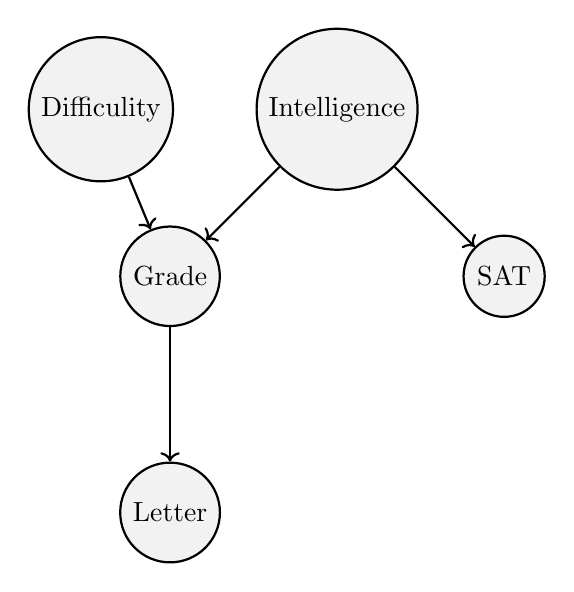
\begin{tikzpicture}[node distance={30mm}, thick, main/.style = {draw, circle}]
        \node[main] (1) [fill=gray!10] {Intelligence};
        \node[main] (2) [left of=1, fill=gray!10] {Difficulity};
        \node[main] (3) [below left of=1, fill=gray!10] {Grade};
        \node[main] (4) [below right of=1, fill=gray!10] {SAT};
        \node[main] (5) [below of=3, fill=gray!10] {Letter};
        \draw[->] (1) -- (3);
        \draw[->] (2) -- (3);
        \draw[->] (1) -- (4);
        \draw[->] (3) -- (5);
      \end{tikzpicture}
      \item first graph is constructed to mimic the phenomenon, which is the student score: in which the grade is dependent on both D,I, $p(G|D,I)$, and S is dependent on I, $P(S|I)$, recommendation letter is dependent on the grade $P(L|G)$. so in this constructed graph, factorization of the joint distribution $P(D,I,G,S,L)=P(D)P(I|D)P(G|D,I)P(S|D,I,G)P(L|D,I,G,S)$ from the chain rule (see appendix on probabilities). from the graph $P(I|D)=P(I)$, $P(S|D,I,G)=P(S,I)$, $P(L|D,I,G,S)=P(L|G)$, therefor $P(D,I,G,S,L)=P(D)P(I)P(G|D,I)P(S|I)P(L|G)$.
      \item here example for the graph truth table for the probability distributions for example P(D) \begin{tabular}{ |c|c| }
        \hline
        $d^0$ & $d^1$ \\
        \hline
        \hline
        0.6 & 0.4 \\
        \hline
      \end{tabular}, P(I) \begin{tabular} {|c|c| }
        \hline
        $i^0$ & $i^1$ \\
        \hline
        \hline
        0.7 & 0.3 \\
        \hline
      \end{tabular}, P(S) \begin{tabular} { |c|c|c| }
        \hline
        & $s^0$ & $s^1$ \\
        \hline
        \hline
        $i^0$ & 0.95 & 0.05 \\
        \hline
        $i^1$ & 0.2 & 0.8 \\
        \hline
      \end{tabular},  P(G) \begin{tabular} { |c|c|c|c| }
        \hline
        & $g^1$ & $g^2$ & $g^3$  \\
        \hline
        \hline
        $i^0,d^0$ & 0.3 & 0.4 & 0.3 \\
        \hline
        $i^0,d^1$ & 0.05 & 0.25 & 0.7 \\
        \hline
        $i^1,d^0$ & 0.9 & 0.08 & 0.02 \\
        \hline
        $i^1,d^1$ & 0.5 & 0.3 & 0.2 \\
        \hline
      \end{tabular},  P(L) \begin{tabular} {|c|c|c|}
        \hline
        & $l^0$ & $l^1$ \\
        \hline
        \hline
        $g^1$ & 0.1 & 0.9 \\
        \hline
        $g^2$ & 0.4 & 0.6 \\
        \hline
        $g^3$ & 0.99 & 0.01 \\
        \hline
      \end{tabular}
        \item now what is $P(d^0,i^1,g^3,s^1,l^1)$ ? from the last derived equation it's $P(d^0)P(i^1)P(g^3|d^0,i^1)P(s^1|i^1)P(l^1|g^3)$ from the tables it's 0.6*0.3*0.02*0.01*0.8.
      \end{description}
    \item A Basyesian network is a directed a-cyclic graph (DAG) such that each node of the graph is a representation of the underlying random variable. such that for each node $X_i$ (random variable) a CPD is $P(X_i|Par_G(X_i))$ where $Par_G$ is a function mapping node (i) random variable to it's parent nodes in the directed graph G
    \item the probability distribution at any node with $X_i$ representation is $P(X_1,..,X_n)=\prod_i{P(X_i|Par_G(X_i))}$ (chain rule see the appendix).
    \item BN distribution build off probability distribution P is expected to be $ P > 0 $, and $\sum {P} = 1$. for example in the prior example $\sum_{D,I,G,S,L}P(D,I,G,S,L)=1$.
    \item Probability P factorizes over G $\iff$ it's represented by chain rule.
      \section{Reasoning Patterns on BN}
      \begin{description}
      \item \textbf{Causal reasoning}: is is reasoning from bottom up, for example $P(l^1) \approx 0.5$,  $P(l^1 | i^0) \approx 0.39$,  $P(l^1 | i^0,d^0) \approx 0.51$.
      \item \textbf{Evidential Reasoning}: is top down reasoning toward the parent nodes, in a class where student gets C with initial $P(i^1)=0.3$, $P(d^1)=0.4$, then the hypothesis that the student is smart given the grades  $P(i^1 |g^3)\approx 0.08$ goes down, and the hypothesis that the class is difficult given the grade  $P(d^1|g^3)\approx 0.63$ goes up.
      \item \textbf{Intercausal Reasoning}: in relational evidential reasoning, for example what is the probability of the intelligence of a student given the grade, and that the it was difficult $P(i^1|g^3,d^1)\approx 0.11$ it went up from 0.08.
        \section{Flow of Probabilistic Influence}
        \begin{description}
        \item it was discussed in previous section that both causal reasoning, and evidential reasoning between the parent, and child node influence each others directly, for example for X, Y variables $ X \rightarrow Y $ e causally affect Y, and $ X \leftarrow Y $ evidentially affect Y. similarly in presence of via node in the case of $X \rightarrow W \rightarrow Y$, then X influences Y via W, similarly $X \leftarrow W \leftarrow Y$ then X influences Y.
        \item in the case in direct edges via nodes even from the same graphical level, for example $ X \leftarrow W \rightarrow Y$ this can be reduced to $ X \leftarrow W $ then X influences W, and $ W \rightarrow Y$ then W influences Y, therefore X influences Y, in the student example the observation of the sat score influences the grade.
        \item meanwhile in the case of \textbf{V-structure} $ X \rightarrow W \leftarrow Y $  in this case X influences W, and Y influences W, but X, doesn't influence Y.
        \end{description}
        \section{d-separation}
        \begin{description}
        \item X, and Y are d-separated in the graph G, if there is no flow of influence between them, and it's denoted by $d-sep_G(X,Y|Z)$, interpreted as X, and Y are separated on the graph G, or there is no flow of influence between them.
        \item to look for active trails, we search the graph from V-structures.
        \item (TODO add illustrative graph)
        \item If P factorizes over G, and $d-sep_G(X,Y|Z)$ then P satisfies $(X \perp Y|Z)$. if there is d-separation between X, and Y given Z, then there is no flow of influence given Z, and from definition of independence $P(X \perp Y | Z) = P(X|Z)P(Y|Z)$.
        \item chain rule expansion of $P(D,I,G,S,L)=P(D)P(I|D)P(G|I,D)P(S|G,I,D)P(L|S,G,I,D)$ from flow of influences in G it reduces to $$P(D)P(I)P(G|D,I)P(S|I)P(L|G)$$
        \item $$P(D,S)=\sum_{G,L,I}P(D)P(I)P(G|D,I)P(S|I)P(L|G)$$
        \item $$=\sum_{I}P(D)P(I)P(S|I)\sum_{G}(P(G|D,I)\sum_{L}(L|G))$$
        \item $$=P(D)(\sum_IP(I)P(S|I))$$
        \item $$=P(D)P(S)=\phi_1(D)\phi_2(S)$$
        \item then $P \models D \perp S$
        \item any node is d-separated from it's non-descendants given it's parents, that is the same rule used to simplify the chain rule joint distribution of the graph G.
          \subsection{I-map}
          \begin{description}
          \item d-separation in G $\rightarrow$ satisfies corresponding independence: $$ I(G) = {(X \perp Y | Z) : d-sep_G(X,Y|Z), X,Y,Z \in G} $$
          \item if P satisfies I(G) then G is an I-map (independency map) of P.
          \item if G is an I-map for P, then P factorizes over G.


          \end{description}
        \end{description}
      \end{description}
    \end{description}
  \end{description}
  \section{Naive Bayes Model}
  \begin{description}
  \item naive base is a graph of independent Variables mapping to the  same parent.
  \item 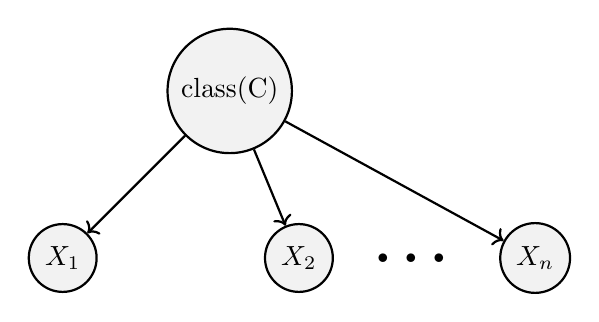
\begin{tikzpicture}[node distance={30mm}, thick, main/.style = {draw, circle}]
    \node[main] (1) [fill=gray!10]  {class(C)};
    \node[main] (2) [below left of=1, fill=gray!10]  {$X_1$};
    \node[main] (3) [right of=2, fill=gray!10]  {$X_2$};
    \node[main] (4) [right of=3, fill=gray!10]  {$X_n$};
    \draw[->] (1) -- (2);
    \draw[->] (1) -- (3);
    \draw[->] (1) -- (4);
    \path (3) -- (4) node[midway,scale=2,font=\bfseries] {\dots};
  \end{tikzpicture}

  \item $$(X_i \perp X_j | C) \forall X_i,X_j$$
  \item $$P(C,X_1,\dots,X_n) = P(C) \prod_{i=1}^{n}P(X_i|C) $$
  \item given two observations of the input features X, we can define the ratio probability of outcome of two observation: $$
    \frac{P(C=c^1 | x_1,\dots,x_n)}{P(C=c^2 | x_1,\dots,x_n)} = \frac{P(C=c^1)}{P(C=c^2)}\prod_{i=1}^n\frac{P(x_i|C=c^1)}{P(x_i|C=c^2)}$$ (note the first term denoted by the prior, and the second is the odd ratio).

  \end{description}
  \section{Template Model}
  \begin{description}
  \item in real world phenomenons, it's always the case that Bayesian representation of a single isolated example is part of larger interconnected network, with shared features, or parameters, for example in NLP sequence model, the previous word, or character influences the current word/character, even the following sequence can resolve the function of current verb, or identity of the none (in named entity recognition for example), similarly in genetic inheritance model, the phenotypes, and genotypes are shared between different branches of wider family, in robot localization, the current position is influenced by control input, prior speed, and position, in image recognition, it's redundant to create a model for each pixel, but rather through is build off the principle of super pixels, where a blob of pixels with shared features are mapped together into a single network.
  \item A template variable $X(u_1,\dots,u_k)$ is instantiated multiple times, for example the location in robot localization at specific time step, person's genotypes, pixel in a blob, or segment, etc.
    \subsection{Distribution over Trajectories}
    \begin{description}
    \item  the Template Model is based of time sequence, or distribution over the trajectory as function of time, with time granularity $\Delta$, such that $X^{(t)}$ is the value of X at time $\Delta{t}$. $X^{(t:t')} = { X^{(t)},\dots,X^{(t')}} (t \leq t')$
    \end{description}
    \subsection{Markov chain}
    \begin{description}
    \item  in a network with trajectory of time $\Delta{t}$ at state $X^{(0:T)}$ with probability: $$P(X^{(0:T)}=P(X^{(0)})\prod_{t=0}^{T-1}P(X^{(t+1)}|X^{(0:t)})$$
    \item the markov assumption is that the state at time $t+1$ is independent of previous states in the interval $[0\text{-}(t-1)]$ given the state at time t, or $$(X^{(t+1)}\perp X^{(0:t-1)} | X^{(t)})$$.
    \item  this assumption can be generalized in the following statement \textbf{``once you Know your present, the past doesn't Matter!''}
    \item thus we can simplify the first equation into: $$P(X^{(0:T)}=P(X^{(0)})\prod_{t=0}^{T-1}P(X^{(t+1)}|X^{(t)})$$
    \item but you should accept this assumption with a grain of salt, so if the current state doesn't capture he past in full, in this case, this assumption breaks, for example future state of robot position is dependent not just of the position, but velocity as well.
    \item so only the likelihood $P(X^{(t+1)}|X^{(t)})=P(X'|X)$ and the prior $P(X^{(0)})$ on the interval $[0\text{-}T]$ determine the following state, being \textbf{Invariant to the time}.
    \item the edges between different time steps are coined:\begin{enumerate}
    \item \textbf{Intra-time slice: } the edges the the same time $t$
    \item \textbf{inter-time slice: } the edges between time t, and time t+1.
    \item \textbf{persistence-time slice: } is inter-time slice but between the same state variables.
    \end{enumerate}
      \subsection{Dynamic Bayesian Network DBN}
      \begin{description}
      \item Dynamics network is a generalization of a template model Bayesian network defined in trajectory of time steps of arbitrary range, where next state model defined in terms of current states, and priors.
      \end{description}
    \end{description}
    \subsection{Hidden Markov Model (HMM)}
    \begin{description}
    \item \textbf{HMMs} are subclass of \textbf{DBNS} with hidden edges either from each state to itself, or from the state at time $t_i$ to arbitrary time $t_j$.
    \item HMM start from state X to X' through a transition state, and outputs an observation at X', through the HMM network, transition, and observation are wrapped in two matrices Transition, and Observation matrices. (we will elaborate more on that in following chapters)
    \item (TODO add a graph)
    \end{description}

  \end{description}
  \section{Structured CPD}
  \begin{description}
  \item previously used tabular representation of the CPD isn't suitable for large network, with node parented by large number of parent nodes, any representation satisfies the general definition would suffice.
  \item a general CPD $P(X|Y_1,\dots,Y_n)$ specifies distribution over X, for each assignment $Y_1,\dots,Y_2$ can use any function to specify a factor $\phi(X,Y_1,\dots,Y_n)$ such that $\sum_x\phi(X,Y_1,\dots,Y_n)=1$ for all $Y_i,\dots,Y_n$.
  \item under the general form, usually there are different models used for example:\begin{enumerate}
  \item Deterministic: is set of $Y_1,\dots,Y_2$  random variables.
  \item Tree-structured: is conditional CPD.
  \item Logistic: logistic activation of the variables.
  \item Noise OR/AND: noise CPD variables.
  \item Linear Gaussian: continuous variable CPD.

  \end{enumerate}
  \item context-specific independence: for two independent variables X, Y given Z, are called context independent given context c, where the context is some condition, defined by a function, then CPD satisfies: $$ (X\perp_c Y | Z,c) $$. examples on this will be in the Tree CPD.

    \subsection{Tree CPD}
    \begin{description}
      %TODO fix this graph weight!!
      \tikzstyle{weight} = [font=\scriptsize]
      \tikzstyle{arrow} =[draw,thick,->]
    \item  \begin{tikzpicture}[node distance={30mm}, thick, main/.style = {draw, circle}, val/.style = {draw, rectangle}]

      \node[main] (1) [fill=gray!10] {\textbf{Apply}};
      \node[main] (2) [below right of=1, fill=gray!10] {\textbf{Sat}};
      \node[val] (3) [below left of=1] {(0.8,0.2)};
      \node[val] (4) [below right of=2] {(0.1,0.9)};
      \node[main] (5) [below left of=2, fill=gray!10] {\textbf{Letter}};
      \node[val] (6) [below right of=5] {(0.4,0.6)};
      \node[val] (7) [below left of=5] {(0.9,0.1)};

      \path[arrow] (1) --  node[weight] {\textbf{$a^1$}} (2);
      \draw[->] (1) -- node[weight] {\textbf{$a^0$}} (3);

      \draw[->] (2) -- node[weight] {\textbf{$s^1$}} (4);
      \draw[->] (2) -- node[weight] {\textbf{$s^0$}} (5);

      \draw[->] (5) -- node[weight] {\textbf{$l^1$}} (6);
      \draw[->] (5) -- node[weight] {\textbf{$l^0$}} (7);
    \end{tikzpicture}

    \item in the previous student example, let's add two nodes, Apply (probability of the student applying for a job), and Job(probability of getting a job), in presence of Sat node, and Letter node.
    \item \textbf{Tree CPD} is CPD with dependencies, and possibly context-specific in-dependencies, on each node's parents, thus flow passes from the parent to child node.
      \item this graph is called \textbf{context-specific CPD Tree} representation of the GPD graph we first discussed.
    \item in this example there  context-specific in-dependencies: \begin{enumerate}
    \item $J\perp_cL|a^1,s^1$
    \item $J\perp_cL,S|a^0$
    \item $J\perp_cL|s^1,A$
    \end{enumerate}
    \item another example, assume in the case that the student have two letters:
    \item  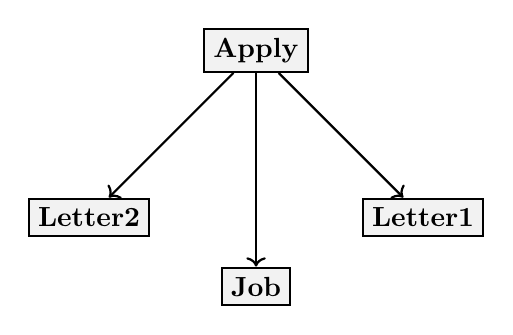
\begin{tikzpicture}[node distance={30mm}, thick, main/.style = {draw, circle}, val/.style = {draw, rectangle}]

      \node[val] (1) [fill=gray!10] {\textbf{Apply}};
      \node[val] (2) [below right of=1, fill=gray!10] {\textbf{Letter1}};
      \node[val] (3) [below left of=1, fill=gray!10] {\textbf{Letter2}};
      \node[val] (4) [below of=1, fill=gray!10] {\textbf{Job}};

      \draw[->] (1) -- (2);
      \draw[->] (1) -- (3);
      \draw[->] (1) -- (4);
    \end{tikzpicture}
    \item this graph would map to the following context-specific CPD
    \item  \begin{tikzpicture}[node distance={30mm}, thick, main/.style = {draw, circle}, val/.style = {draw, rectangle}]

      \node[main] (1) [fill=gray!10] {\textbf{Apply}};
      \node[main] (2) [below right of=1, fill=gray!10] {\textbf{Letter2}};
      \node[main] (3) [below left of=1, fill=gray!10] {\textbf{Letter1}};
      \node[val] (5) [below right of=2] {(0.1,0.9)};
      \node[val] (4) [left of=5] {(0.8,0.2)};

      \node[val] (7) [below left of=3] {(0.9,0.1)};
      \node[val] (6) [right of=7] {(0.3,0.7)};

      \path[arrow] (1) --  node[weight] {\textbf{$a^2$}} (2);
      \draw[->] (1) -- node[weight] {\textbf{$a^1$}} (3);

      \draw[->] (2) -- node[weight] {\textbf{$l^1$}} (4);
      \draw[->] (2) -- node[weight] {\textbf{$l^0$}} (5);

      \draw[->] (3) -- node[weight] {\textbf{$l^1$}} (6);
      \draw[->] (3) -- node[weight] {\textbf{$l^0$}} (7);
    \end{tikzpicture}
    \item in this case $(L1\perp_cL1|J,A)$
      \subsection{Multiplexer CPD}
      \begin{description}
      \item .
      \end{description}
    \end{description}

  \end{description}



  \chapter{Natural language processing}
  \section{pre-processing}
  \begin{description}
  \item the problem here is how to extract features $\mathbf{X}$ from the a sentence.
  \item for example how to classify a sentence being positive, or negative, assigning 0 for negative, and 1 for positive, starting for a preprocessed sentence how to turn it into a feature set X.
  \item but there are unnecessary punctuation, conjugation, and stops that need to be get rid of, so first we need to pre-process our data-set as follows:
    \begin{enumerate}
    \item iliminate handles and URLs
    \item tokenize the string into words
    \item remove stop words such as ``and, is, a, on, etc''
    \item covert every word into it's stem form
    \item lower case transformation
    \end{enumerate}

  \end{description}
  \section{Example: positive, negative classifier}
  \begin{description}
  \item given sentence s=``i love NLP, therefore i study it'' how to classify s=['i', 'love', 'NLP', ',', 'therefore', 'i', 'study', 'it']  as positive or negative?.
  \item for a set of strings $S=\{s_1, s_2, .., s_n\}$, matching each string against a vocabulary of all words to end up with two vectors of word frequency, we create positive frequency vector freqs(w,1), and negative frequency vector freqs(w,0) such that w stand for sentence word, and such that $X_m=[1, \sum_{w}freqs(w,1), \sum_{w}freqs(w,0)]$
  \item given a set of sentences, each is labeled for training as either positive, or negative. we mark each word in a positive-labeled sentence as positive, even if the word is negative, and conversely the opposite with negative-labeled sentences, we mark every word as negative.
\item first of all we create a set vocabulary $V$ that includes all sets, or sentences $S$, $V=\{words(s_i) | s_i \in{S}\}$.
\item for example in training sets ${s_1, s_2}$, $s_1$=''i love NLP, therefore i study it'' labeled as positive, and $s_2$=''society no longer in need for black magic, or superstition'' labeled negative, we can extract pos-neg features against vocabulary V=['i', 'love', 'NLP', ',', 'therefore', 'study', 'it', 'society', 'no', 'longer', 'in', 'need', 'for', 'black', 'magic', 'or', 'superstition'], pos-freqs = [2, 1, 1, 1, 1, 1, 1, 0, 0, 0, ..., 0], neg-freqs = [0, 0, 0, 1, 0, 0, 0, 1, 1, 1, 1, 1, 1, 1, 1, 1, 1]. $X_m$=[1, 8, 11]. for m training sets, $X_{m}=\begin{vmatrix}1&x_1^{(1)}&x_2^{(1)}\\1&x_1^{(2)}&x_2^{(2)}\\1&x_1^{(3)}&x_2^{(3)}\\...\\1&x_1^{(m)}&x_2^{(m)}\end{vmatrix}$pp
  \end{description}
\section{Logistic regression classifier}
\begin{description}
\item let's see how this fits inside the Gradient Descent algorithm, for $\sigma(X^i, \theta^i)=\frac{1}{1+e^{-z}}$, we add the bias b to the $X^i$ itself, and therefore $z=\theta^TX^i$.
\item therefore for a positive z we get  $\sigma>0.5$, and inversely for negative z we have $\sigma<0.5$.
\item now we ready for Gradient Descent, given initial parameters $\theta$, we predict, or evaluate the logistic:
\item$\sigma(X^i, \theta_j)$, then loss function $L(\hat{y}, y)=-[\hat{y}log(\hat{y}) + (1-y)log(1-\hat{y})]$, gradient $\nabla=\partial{J}/\partial{\theta_j} = \frac{X^T}{m}(\hat{y} - y)$, updating $\theta_j := \theta_j - \alpha\nabla$. iterate through gradient descent k times.
\end{description}

\section{Naive Bayes classifier}
\begin{description}
\item The priorpp probability represents the underlying probability in the target population that a tweet is positive versus negative.  In other words, if we had no specific information and blindly picked a tweet out of the population set, what is the probability that it will be positive versus that it will be negative? That is the "prior".

\item The prior is the ratio of the probabilities $\frac{P(D_{pos})}{P(D_{neg})}$.
\item We can take the log of the prior to rescale it, and we'll call this the logprior

\item $$\text{logprior} = log \left( \frac{P(D_{pos})}{P(D_{neg})} \right) = log \left( \frac{D_{pos}}{D_{neg}} \right)$$.

\item Note that $log(\frac{A}{B})$ is the same as $log(A) - log(B)$.  So the logprior can also be calculated as the difference between two logs:

\item $\text{logprior} = \log (P(D_{pos})) - \log (P(D_{neg})) = \log (D_{pos}) - \log (D_{neg})$

\item To compute the positive probability and the negative probability for a specific word in the vocabulary, we'll use the following inputs:

\item $freq_{pos}$ and $freq_{neg}$ are the frequencies of that specific word in the positive or negative class. In other words, the positive frequency of a word is the number of times the word is counted with the label of 1.

\item $N_{pos}$ and $N_{neg}$ are the total number of positive and negative words for all documents (for all tweets), respectively.
- $V$ is the number of unique words in the entire set of documents, for all classes, whether positive or negative.

\item We'll use these to compute the positive and negative probability for a specific word using this formula:

\item $$ P(W_{pos}) = \frac{freq_{pos} + 1}{N_{pos} + V}$$
\item $$ P(W_{neg}) = \frac{freq_{neg} + 1}{N_{neg} + V}$$

\item Notice that we add the "+1" in the numerator for additive smoothing.

\item To compute the loglikelihood of that very same word, we can implement the following equations:

\item $$\text{loglikelihood} = \log \left(\frac{P(W_{pos})}{P(W_{neg})} \right)$$

\item $$ p = logprior + \sum_i^N (loglikelihood_i)$$

\item Some words have more positive counts than others, and can be considered "more positive".  Likewise, some words can be considered more negative than others.
\item One way for us to define the level of positiveness or negativeness, without calculating the log likelihood, is to compare the positive to negative frequency of the word.
\item Note that we can also use the log likelihood calculations to compare relative positivity or negativity of words.
\item We can calculate the ratio of positive to negative frequencies of a word.
\item Once we're able to calculate these ratios, we can also filter a subset of words that have a minimum ratio of positivity / negativity or higher.
\item Similarly, we can also filter a subset of words that have a maximum ratio of positivity / negativity or lower (words that are at least as negative, or even more negative than a given threshold).

\item $$ \text{ratio} = \frac{pos_{words} + 1}{neg_{words} + 1} $$

\item In prevision section a Logistic regression classified, but we can quick solve the same problem in much simpler algorithm through the evaluation of the likelihood of a sentence being positive matched against given Vocabulary table $V$.
\item Recall that conditional probability $p(w_i|pos) = \frac{p(w_i\cap{pos})}{p(pos)}$, $p(pos)=freq(pos)/total$, $p(w_i\cap{pos})=freq(w_i)/total$, then $p(w_i|pos)=freq(w_i)/freq(pos)$
\item Likelihood of a positive is defined as $\prod_{i=1}^{m}{\frac{p(w_i|pos)}{p(w_i|neg)}}$, if likelihood $>$ 1 then sentence is positive, otherwise, it's negative.
\item to reduce the sensitivity of each word, and avoid getting 0 $p(w_i|class)$, $class\in \{pos, neg\}$ we modify the conditional probabilistic frequency using the so-called 'laplacian smoothing': $p(w_i|class)=\frac{freq(w_i|class)+1}{freq(class)+unique(V)}$, freq(class) is defined as $N_{class}$, and unique(V) is defined as $N_V$, for example $p(w_i|pos)=\frac{freq(w_i|pos)+1}{N_{pos}+N_V}$.
\item to keep the scale small as possible likelihood is replaced with log of likelihood coined with symbol $\lambda(w_i)=log(\frac{p(w_i|pos)}{p(w_i|neg)})$, and a prior=$log(\frac{p(pos)}{p(neg)})$, the classifier of a sentence $W$ is equivalent to prior + $\sum_{i=1}^{m}{\lambda{w_i}}$, and if $\lambda>0$ then it's positive, and negative otherwise.
\end{description}
\section {cosine similaritis}
\begin{description}

\item The cosine similarity function is:

\item $$\cos (\theta)=\frac{\mathbf{A} \cdot \mathbf{B}}{\|\mathbf{A}\|\|\mathbf{B}\|}=\frac{\sum_{i=1}^{n} A_{i} B_{i}}{\sqrt{\sum_{i=1}^{n} A_{i}^{2}} \sqrt{\sum_{i=1}^{n} B_{i}^{2}}}$$

\item $A$ and $B$ represent the word vectors and $A_i$ or $B_i$ represent index i of that vector.
\item Note that if A and B are identical, you will get $cos(\theta) = 1$.
\item Otherwise, if they are the total opposite, meaning, $A= -B$, then you would get $cos(\theta) = -1$.
\item If you get $cos(\theta) =0$, that means that they are orthogonal (or perpendicular).
\item Numbers between 0 and 1 indicate a similarity score.
\item Numbers between -1-0 indicate a dissimilarity score.
\end{description}
\subsection {Euclidean distance}
\begin{description}
  \item You will now implement a function that computes the similarity between two vectors using the Euclidean distance.
Euclidean distance is defined as:

\item $$ \begin{aligned} d(\mathbf{A}, \mathbf{B})=d(\mathbf{B}, \mathbf{A}) &=\sqrt{\left(A_{1}-B_{1}\right)^{2}+\left(A_{2}-B_{2}\right)^{2}+\cdots+\left(A_{n}-B_{n}\right)^{2}} \\ &=\sqrt{\sum_{i=1}^{n}\left(A_{i}-B_{i}\right)^{2}} \end{aligned}$$

\item $n$ is the number of elements in the vector
\item $A$ and $B$ are the corresponding word vectors.
\item The more similar the words, the more likely the Euclidean distance will be close to 0.p
\end{description}

\section {Principle Component Analysis (PCA)}
\begin{description}
\item PCA is a method that projects our vectors in a space of reduced dimension, while keeping the maximum information about the original vectors in their reduced counterparts. In this case, by *maximum infomation* we mean that the Euclidean distance between the original vectors and their projected siblings is minimal. Hence vectors that were originally close in the embeddings dictionary, will produce lower dimensional vectors that are still close to each other.

\item such that similar words will be clustered next to each other. For example, the words 'sad', 'happy', 'joyful' all describe emotion and are supposed to be near each other when plotted. The words: 'oil', 'gas', and 'petroleum' all describe natural resources. Words like 'city', 'village', 'town' could be seen as synonyms and describe a

\item Before plotting the words, you need to first be able to reduce each word vector with PCA into 2 dimensions and then plot it. The steps to compute PCA are as follows:
  \begin{itemize}
  \item Mean normalize the data
  \item Compute the covariance matrix of the data ($\Sigma$).
  \item Compute the eigenvectors and the eigenvalues of your covariance matrix
  \item Multiply the first K eigenvectors by the normalized data.
\end{itemize}
\end{description}

\section {Machine Translation}
\begin{description}

\item Given dictionaries of English and French word embeddings you will create a transformation matrix `R`
\item Given an English word embedding, $\mathbf{e}$, you can multiply $\mathbf{eR}$ to get a new word embedding $\mathbf{f}$.
\item Both $\mathbf{e}$ and $\mathbf{f}$ are row vectors.
\item we can then compute the nearest neighbors to `f` in the french embeddings and recommend the word that is most similar to the transformed word embedding.

\item Find a matrix `R` that minimizes the following equation.

\item $$\arg \min _{\mathbf{R}}\| \mathbf{X R} - \mathbf{Y}\|_{F} $$

\item The Frobenius norm of a matrix $A$ (assuming it is of dimension $m,n$) is defined as the square root of the sum of the absolute squares of its elements:

\item $$\|\mathbf{A}\|_{F} \equiv \sqrt{\sum_{i=1}^{m} \sum_{j=1}^{n}\left|a_{i j}\right|^{2}}$$


\item In the real world applications, the Frobenius norm loss:

\item $$\| \mathbf{XR} - \mathbf{Y}\|_{F}$$

\item is often replaced by it's squared value divided by $m$:

\item $$ \frac{1}{m} \|  \mathbf{X R} - \mathbf{Y} \|_{F}^{2}$$

\item where $m$ is the number of examples (rows in $\mathbf{X}$).

\item The same R is found when using this loss function versus the original Frobenius norm.
\item The reason for taking the square is that it's easier to compute the gradient of the squared Frobenius.
\item The reason for dividing by $m$ is that we're more interested in the average loss per embedding than the  loss for the entire training set.
\item The loss for all training set increases with more words (training examples),
\item so taking the average helps us to track the average loss regardless of the size of the training set.
\end{description}
\subsection {Loss function L}
\begin{description}
\item The loss function will be squared Frobenoius norm of the difference between
\item matrix and its approximation, divided by the number of training examples $m$.
\item  Its formula is:
\item $$ L(X, Y, R)=\frac{1}{m}\sum_{i=1}^{m} \sum_{j=1}^{n}\left( a_{i j} \right)^{2}$$

\item where $a_{i j}$ is value in $i$th row and $j$th column of the matrix $\mathbf{XR}-\mathbf{Y}$.

\item The norm is always nonnegative (we're summing up absolute values), and so is the square.
\item When we take the square of all non-negative (positive or zero) numbers, the order of the data is preserved.
\item For example, if $3 > 2, 3^2 > 2^2$
\item Using the norm or squared norm in gradient descent results in the same location of the minimum.
\item  Squaring cancels the square root in the Frobenius norm formula. Because of the chain rule, we would have to do more calculations if we had a square root in our expression for summation.
\item Dividing the function value by the positive number doesn't change the optimum of the function, for the same reason as described above.
\item We're interested in transforming English embedding into the French. Thus, it is more important to measure average loss per embedding than the loss for the entire dictionary (which increases as the number of words in the dictionary increases).
\end{description}
\subsection {gradient descent}
\begin{description}
\item Calculate the gradient of the loss with respect to transform matrix `R`.
\item The gradient is a matrix that encodes how much a small change in `R` affect the change in the loss function.
\item The gradient gives us the direction in which we should decrease `R`
\item to minimize the loss.
\item $m$ is the number of training examples (number of rows in $X$).
\item The formula for the gradient of the loss function $L(X,Y,R)$ is:
\item $$\frac{d}{dR}L(X,Y,R)=\frac{d}{dR}\Big(\frac{1}{m}\| X R -Y\|_{F}^{2}\Big) = \frac{2}{m}X^{T} (X R - Y)$$

\subsection{fixed number of iterations}
\item You cannot rely on training loss getting low -- what you really want is the validation loss to go down, or validation accuracy to go up. And indeed - in some cases people train until validation accuracy reaches a threshold, or -- commonly known as "early stopping" -- until the validation accuracy starts to go down, which is a sign of over-fitting.
\item Why not always do "early stopping"? Well, mostly because well-regularized models on larger data-sets never stop improving. Especially in NLP, you can often continue training for months and the model will continue getting slightly and slightly better. This is also the reason why it's hard to just stop at a threshold -- unless there's an external customer setting the threshold, why stop, where do you put the threshold?
\item Stopping after a certain number of steps has the advantage that you know how long your training will take - so you can keep some sanity and not train for months. You can then try to get the best performance within this time budget. Another advantage is that you can fix your learning rate schedule -- e.g., lower the learning rate at 10% before finish, and then again more at 1% before finishing. Such learning rate schedules help a lot, but are harder to do if you don't know how long you're training.

\item  Pseudocode:
\item 1. Calculate gradient $g$ of the loss with respect to the matrix $R$.
\item 2. Update $R$ with the formula:
\item $$R_{\text{new}}= R_{\text{old}}-\alpha g$$
\item Where $\alpha$ is the learning rate, which is a scalar.

  \subsection {k-Nearest neighbors algorithm}
\item k-NN is a method which takes a vector as input and finds the other vectors in the dataset that are closest to it.
\item The 'k' is the number of "nearest neighbors" to find (e.g. k=2 finds the closest two neighbors).

  \subsection{Searching for the translation embedding}

\item Since we're approximating the translation function from English to French embeddings by a linear transformation matrix R
, most of the time we won't get the exact embedding of a French word when we transform embedding e

\item of some particular English word into the French embedding space.

\item This is where k-NN becomes really useful! By using 1-NN with eR as input, we can search for an embedding f (as a row) in the matrix Y which is the closest to the transformed vector eR.

\item  Note: Distance and similarity are pretty much opposite things.
\item We can obtain distance metric from cosine similarity, but the cosine similarity can't be used directly as the distance metric.
\item When the cosine similarity increases (towards $1$), the "distance" between the two vectors decreases (towards $0$).
\item We can define the cosine distance between $u$ and $v$ as
\item $$d_{\text{cos}}(u,v)=1-\cos(u,v)$$

  \subsection{LSH and document search}
\item In this part of the assignment, you will implement a more efficient version of k-nearest neighbors using locality sensitive hashing. You will then apply this to document search.

\item Process the tweets and represent each tweet as a vector (represent a document with a vector embedding).
\item Use locality sensitive hashing and k nearest neighbors to find tweets that are similar to a given tweet.
\item we will now implement locality sensitive hashing (LSH) to identify the most similar tweet.
\item Instead of looking at all 10,000 vectors, you can just search a subset to find its nearest neighbors
\item we can divide the vector space into regions and search within one region for nearest neighbors of a given vector.

\subsection{Bag-of-words (BOW) document models}
\item Text documents are sequences of words.
\item The ordering of words makes a difference. For example, sentences "Apple pie is
\item better than pepperoni pizza." and "Pepperoni pizza is better than apple pie"
\item have opposite meanings due to the word ordering.
\item However, for some applications, ignoring the order of words can allow
\item us to train an efficient and still effective model.
\item This approach is called Bag-of-words document model.

\item Document embedding is created by summing up the embeddings of all words
in the document.
\item If we don't know the embedding of some word, we can ignore that word.

\subsection{ Choosing the number of planes}

\item Each plane divides the space to $2$ parts.
\item So $n$ planes divide the space into $2^{n}$ hash buckets.
\item We want to organize 10,000 document vectors into buckets so that every bucket has about $~16$ vectors.
\item For that we need $\frac{10000}{16}=625$ buckets.
\item We're interested in $n$, number of planes, so that $2^{n}= 625$. Now, we can calculate $n=\log_{2}625 = 9.29 \approx 10$.

\item  In $3$-dimensional vector space, the hyperplane is a regular plane. In $2$ dimensional vector space, the hyperplane is a line.
\item Generally, the hyperplane is subspace which has dimension $1$ lower than the original vector space has.
\item A hyperplane is uniquely defined by its normal vector.
\item Normal vector $n$ of the plane $\pi$ is the vector to which all vectors in the plane $\pi$ are orthogonal (perpendicular in $3$ dimensional case).
\subsection{ Getting the hash number for a vector}

\item For each vector, we need to get a unique number associated to that vector in order to assign it to a "hash bucket".

\item Using Hyperplanes to split the vector space:
\item We can use a hyperplane to split the vector space into $2$ parts.
\item  All vectors whose dot product with a plane's normal vector is positive are on one side of the plane.
\item All vectors whose dot product with the plane's normal vector is negative are on the other side of the plane.

\item Encoding hash buckets:
\item For a vector, we can take its dot product with all the planes, then encode this information to assign the vector to a single hash bucket.
\item When the vector is pointing to the opposite side of the hyperplane than normal, encode it by 0.
\item Otherwise, if the vector is on the same side as the normal vector, encode it by 1.
\item If you calculate the dot product with each plane in the same order for every vector, you've encoded each vector's unique hash ID as a binary number, like [0, 1, 1, ... 0].

\item hash algorithm:

\item We've initialized hash table `hashes` for you. It is list of $N_{universe}$ matrices, each describes its own hash table. Each matrix has $N_{dims}$ rows and $N_{planes}$ columns. Every column of that matrix is a $N_{dims}$ dimensional normal vector for each of $N_{planes}$ hyperplanes which are used for creating buckets of the particular hash table.

\item  First multiply your vector `v`, with a corresponding plane. This will give you a vector of dimension $N_{planes}$.
\item You will then convert every element in that vector to 0 or 1.
\item You create a hash vector by doing the following: if the element is negative, it becomes a 0, otherwise you change it to a 1.
\item You then compute the unique number for the vector by iterating over $N_{planes}$
\item Then you multiply $2^i$ times the corresponding bit (0 or 1).
\item You will then store that sum in the variable $hash_{value}$.
\item $$ hash = \sum_{i=0}^{N-1} \left( 2^{i} \times h_{i} \right) $$

\end{description}
\section{Probabilistic model of pronounciation and spelling}
\begin{description}
  \subsection{auto-correction}
\item the misspelling is quite common in writing, and to transduct a word from the misspelled form to dictionary closest word, most relevant to the context for spelling, and pronunciation we utilize \textbf{Bayes Rule}, and \textbf{the noisy channel model}, and this problem can be divided into two categories:
\item 1. word error detection: in which the algorithm is run on the word in isolation.
\item 2. context error detection: where correction take place in a specific context.
\item 80\% of the misspelled words are caused by single-eror misspellings: can be divided into four categories:
  \begin{itemize}
  \item insertion: mistyping the as ther
  \item deletion: mistyping the as th
  \item substitution: mistyping the as thw
  \item transposition mistyping the as hte
  \end{itemize}
  \subsection{Bayesian inference model}
\item given a noisy word through noisy channel, \textbf{O} as our observation, we need to match it to the nearest word in the dictionary.
\item we build a vocabulary \textbf{V}, and our model ought to map noisy \textbf{O} to \textbf{$\hat{w}$}.
\item $$ \hat{w}=\underset{w \in V}{\operatorname{argmax}}P(w|O) $$
\item $$ \hat{w}=\underset{w \in V}{\operatorname{argmax}}\frac{P(O|w)P(w)}{P(O)} $$
\item since we iterate through the whole word set in the vocabulary \textbf{V} P(O) is fixed, and we can ignore it, then:
\item $$ \hat{w}=\underset{w \in V}{\operatorname{argmax}} P(O|w)P(w) $$
\item where P(w) is the \textbf{prior}, P(O|w) is the \textbf{likelihood} function.
\item p(w) is the word frequency: $\frac{frequency(w)}{size of the corpus}$, to avoid getting zero frequency we use Laplacian smoothing:
\item $$ p(w)=\frac{freq(w)+1}{N+V} $$ such that V is the size of vocabulary in this context, and N is the size of the corpus.
\item there different algorithms for error correction, and processing, among those are \textbf{minimum edit distance}, \textbf{Viterbi} \textbf{forward}, \textbf{CYK}, \textbf{Earley}.
  \subsection{Minimum edit distance}
\item It's a metric value between different noise channels for the same word, or weight for insertion, deletion, and substitution, weighting each by 1, but substitution by 2 (insertion+substitution), known as \textbf{Levenshtein} distance.
\item given two words target, and source, word distance can be calculated through Dynamic programming, laying out the target of length$\rightarrow{n}$ in the first column, and source of length $\rightarrow{m}$ in the first row, and creating matrix \textbf{distance} of size $\rightarrow{n}$ (n+1,m+1).
\item looping through each column i from 0 $\rightarrow{n}$, and each row j from 0 $\rightarrow{m}$ :
\item $$dstance[i,j] \leftarrow Min \begin{cases} \text{(distance[i-1,j] + inseration-cost($target_j$)}\\ \text{distance[i-1, j-1] + substraction-cost($source_j$,$target_i$)}\\ \text{distance[i,j-1] + insertion-cost($source_j$))}\end{cases}$$
\end{description}

\section {Grammar Weighted Automata}
\begin{description}
\item it's a weighted directed graph of finite automaton for language, to predict the probability of following word.
  \subsection{Markov chain}
    \item .
  \subsection{Hidden Markov Models HMMs}
\item it's a special time of weighted Automata, in which previous states determine the current state.
\item the weights over the directed arrows can be loaded from a given corpus as the probability of word $w_i$ followed by $w_j$, or in case of pronunciation, the probability of phone(p) $p_i$ followed by $p_j$.
\item in tagged words we can classify each word in the corpus into specific group, and build the weighted graph for the classes instead.
\item a weighted automaton is consisting of a set of states $q=<q_0q_1q_2...q_n>$, and transition states $a_{01}a_{12}a_{23}...a_{n-1}a_n$, while the input to the machine is called the Observation and denoted by $O=(o_1o_2o_3...o_t)$.
\item decoding problem: is the resolution of the underlying sequence that produce a certain observation.
\item word-detection is done through Bayesian inference $P(w|O)=P(O|w)p(w)$ if we ignore the denominator as discussed earlier.
\item this method has two important elements first the forward algorithm which is analogous to the Minimum Edit distance algorithm, yet more generalized, the latter can be seen as a special case, in the forward algorithm, the row do no just represent a sequence of characters, but does indicate the possibilities to reach to each state $q_i$ from any previous state, and instead of the calculation of the minimum, here the sum of all probabilities in current state j forward[t,j] after observing the first t observations, given the automaton $\lambda$ of paths that lead to current state of aggregated,or in other words, the likelihood of the observations times the word probability p(w) and this is calculated through multiplying three different factors: \begin{enumerate}
\item previous path probability \textit{forward[t-1,i]}.
\item transition probability $a_{ij}$.
\item observation likelihood $b_{jt}$ that the current state j matches the observation symbol t. can takes the range [0,1], 1 if there is matchs, and 0 otherwise.
\end{enumerate}
\item $$ forward[t,j] = P(o_1,o_2,...,o_t,q_t = j|\lambda)P(w) $$
\item where $q_t = j$ means the probability that the t'th state in the sequence of states is state j (current state).
\item after initializing forward[0,0]=1.
\item $$ forward[j,t] = forward[i,t-1] * a[j,i] *b[j,o_t] $$ (note that i is index of previous state),
\item the problem with Forward algorithm is that it's run through a single channel. There is more efficient graph than that of forward algorithm which enable us to track multiple of words, or sentences moving from state to another, or a more general algorithm called Viterbi.
  \subsection {Viterbi Algorithm}
  \item it's consists of three main steps, \textbf{initialization} of viterbi probability, and path matrix, and viterbi \textbf{forward}, and viterbi \textbf{backward}.
\item it's a variation, or general implementation of the forward algorithm with multiple words/sentences running simultaneously.
\item we set up a probability matrix, where each column is set for time index t, and one row for each state in the Automata graph.
\item each column has a cell for each state $q_i$.
\item the evaluation of the viterbi[t,j] is the same as in the forward algorithm.
\item there is a slight difference with the Forward algorithm, which is the viterbi maximizes the sum of all path to current state.
  \item.

    \subsection {Part of Speech tagging (POS)}
  \item starting with the phenomenon: a single word can have different meanings in different sentences.
  \item How to model such linguistic complexity in language processing?
  \item look at the following examples: \begin{itemize}
    \item The whole team played well. [adverb]
    \item You are doing well for yourself. [adjective]
    \item Well, this assignment took me forever to complete. [interjection]
    \item The well is dry. [noun]
    \item Tears were beginning to well in her eyes. [verb]
  \end{itemize}
  \item the same word is used in different contexts to mean different things with different part of speech tags.

  \item Algorithm:
    \begin{enumerate}

    \item calculate transition counts vector $C_t$ from tag $t_{i-1}$ to $t_i$ to calculate $P(t_i|t_{i-1})$.

    \item calculate emission counts vector $C_e$ of tag $t_i$ and word $w_i$ to calculate $P(w_i|t_i)$.

    \item tag counts is the count $C$ of occurrence of specific tag.

    \item create a Markov model of tag states, of transition probability from step (1), and create \textbf{transition matrix A} of all the sates as follows: $\frac{C_t(t_{i-1},t_i) + \alpha}{C(t_{i-1}) + \alpha N}$ smoothed to avoid zero, or undefined value, or in other words to calculate the probability of the relation that doesn't exis, constant $\alpha$ usually small value of 0.001, and N the number of tags.

    \item create \textbf{emission matrix B} from step(2) for the probability of observation O at specific state t:  $\frac{C_e(t_i, w_i) + \alpha}{C(t_i) + \alpha V}$. where V is the number of words in the dictionary.

    \item the formula for the Viterbi matrix is different in the first column(first word) than the rest of the columns, in the previous column the previous value term is ignored!

    \item Viterbi initialization: the previous value is set to the begining tag (i.e str --s--) let's call it start-state, of index 0, or $start_{idx}$, also to avoid getting zero value we take the logarithm of the natural e, of the transition, and emission states: $log(A[0,j]*log[j,w_i])$ = $log(A[0,j]) + log[j,w_i]$ (where j in the current tag index in the list of tags of size N, and i is the previous state index, and in the case of initialization it's 0,  $j \in N$), therefore the final initialization algorithm is:  $$V[j,0] = log(A[0,j]) + log[j,w_i]$$ $w_i$ is the current state word.

    \item Viterbi forward: $$V[j,i] = \underset{k \in N}{\operatorname{argmax}}(V[k, i-1] + log(A[k,j]) + log[j,w_i])$$

    \item Viterbi backward: starting for the last we pick the highest probability in the Viterbi matrix and record the indices of the corresponding tag, going backward up to the first column, add those tags in reverse order.
    \end{enumerate}


    \section {N-grams}
    \subsection{Smoothing}
    \begin{description}
      \item Add-k smoothing was described as a method for smoothing of the probabilities for previously unseen n-grams.
      \end{description}
    \subsection{Back-off}
    \begin{description}
    \item Back-off is a model generalization method that leverages information from lower order n-grams in case information about the high order n-grams is missing. For example, if the probability of an trigram is missing, use bigram information and so on.
    \end{description}
    \subsection{Interpolation}
    \begin{description}
    \item The other method for using probabilities of lower order n-grams is the interpolation. In this case, you use weighted probabilities of n-grams of all orders every time, not just when high order information is missing.
    \end{description}


\end{description}

\citep{xyz2}
\bibliographystyle{apalike}
\bibliography{bib0}

\begin{appendices}
  \chapter{Introduction to probabilities}
  \section{probabilities chain rule}
  \section {Naive Bayes}
  \chapter{Covariance}
  \chapter{Single Value Decomposition}
  \chapter {Exponentially weighted averages}
  \begin{description}
  \item if we have a stochastic function over vector $\Theta$, to smooths it's overshoot a bit, we can take the averages over a window of size $k$, but for large sized vector $\Theta$, it's expensive to keep all values at memory, and repeatedly run the average function over a small window, instead we can keep just the previous value through weighted averages.
  \item the weighted averages for $\Theta=(\theta^1,\theta^2,...,\theta^n)$ the weighted averaged $theta^i$: $V\theta^i=\beta V \theta^{i-1} + (1-\beta) \theta^i$.
  \item there is a bias in the weighted averages in the initial steps, we can compensate for that through \textbf{bias correction} $V\theta^i=\frac{V\theta^i}{(1-\beta^t)}$. where t is a positive integer of the first initial values, for example if we doing bias correction for the first 10 values, then $t=10$.
    \subsection {How to choose the value $\beta$ ?}
    \begin{description}
    \item it's more efficient to use average function over a window of inputs, but it's expensive in a large input set, in fact the $\beta$ value is a control of window size as it tend to fade away as the exponential gets bigger.
    \item if we expand the $dV\theta^n$: $$
      (1-\beta)\theta^{n} + \beta(1-\beta)^2\theta^{n-1} + ... + \beta(1-\beta)^{n}\theta^1
      $$ and we know that $(1-\beta)^{\frac{1}{\beta}} = \frac{1}{e} = 0.367$ then $\frac{1}{1-\beta}$ iterations this weighting term will be $\frac{1}{e}$, meaning closer to zero, and then we can interpret the weight decay algorithm as the function that take the average over the last $\frac{1}{1-\beta}$ elements.

    \end{description}
  \end{description}
  \chapter{smoothing (add-k, and add-one Laplacian)}
  \begin{description}
    \item .
    \end{description}
  \chapter{Kernels, and Convolution functions}
  \begin{description}
    \item .
    \end{description}
\end{appendices}
\end{document}
